\documentclass[10pt]{article}

%% Packages
\usepackage[margin=1in, top=0.75in]{geometry}
\usepackage[utf8]{inputenc}
\usepackage[T1]{fontenc}
\usepackage[usenames,dvipsnames]{xcolor}
\usepackage{amssymb, amsfonts, amsmath, mathrsfs, enumitem, tcolorbox, bbm, graphicx, fullpage, parskip, mathtools, float, amsthm}
\usepackage{tikz,sgame,bbm,todonotes, setspace, soul, array}
\usepackage[english]{babel}
\usepackage{pdfpages}
\setcounter{tocdepth}{3}
% Links (and references)
\definecolor{linkblue}{RGB}{40, 50, 200}
\usepackage[colorlinks=true, allcolors={linkblue}]{hyperref}

%% Math operators
\newcommand*{\ones}{\text{\usefont{U}{bbold}{m}{n}1}}
\newcommand{\reals}{\mathbb{R}}
\newcommand{\rationals}{\mathbb{Q}}
\newcommand{\integers}{\mathbb{Z}}
\newcommand{\naturals}{\mathbb{N}}
\newcommand{\complex}{\mathbb{C}}
\newcommand{\normal}{\mathcal{N}}

% General math
\newcommand{\abs}[1]{\mathop{\left|#1\right|}} % absolute value
\newcommand{\inv}{^{-1}} % inverse
\let\oldST\st
\newcommand{\strikethrough}{\oldST}
\renewcommand{\st}{\;\text{s.t.}\;} % math operator for "such that"
\newcommand{\eg}{\emph{e.g.} }
\newcommand{\ie}{\emph{i.e.} }
\newcommand{\interior}{\mathop{\rm int}}

% Optimization
\newcommand{\argmax}{\mathop{\rm argmax}}
\newcommand{\argmin}{\mathop{\rm argmin}}
\newcommand{\opt}{^\star}
% Analysis, vector spaces, and topology
\newcommand{\set}[1]{\left\{#1\right\}} % set notation
\newcommand{\seq}[1]{_{#1}^{\infty}} % add sequence notiation to set (or to a summation symbol for series)
\newcommand{\setless}{\mathop{\backslash}} % A \ B notation
\newcommand{\pow}{\mathop{\mathcal{P}}} % power set
\newcommand{\im}{\mathop{\rm im}} % image
\newcommand{\spans}{\mathop{\rm span}} % span
\newcommand{\rank}{\mathop{\rm rank}} % rank
\newcommand{\topo}{\mathop{\mathcal{T}}} % topology
\newcommand{\cont}{\mathop{\bf C}} % continuously differentiable

% Matrices
\newcommand\colvector[1]{\begin{bmatrix}#1\end{bmatrix}}
\newcommand\rowvector[1]{\begin{bmatrix}#1\end{bmatrix}}
\newcommand\matrixc[1]{\begin{bmatrix}#1\end{bmatrix}}
\newcommand\matrixp[1]{\begin{pmatrix}#1\end{pmatrix}}
\newcommand\detmatrix[1]{\begin{vmatrix}#1\end{vmatrix}}
\newcommand\rankmatrix{\begin{bmatrix}I_r & \rvline & \mathbf{0}_1\\\hline \mathbf{0}_2 & \rvline & \mathbf{0}_3 \end{bmatrix}}

% Statistics
\newcommand{\cov}{\mathop{\rm cov}} % covariance
\newcommand{\corr}{\mathop{\rm corr}} % correlation
\newcommand{\expect}{\mathop{\mathbb{E}}} % expectation
\newcommand{\indep}{\perp \hspace{-1.4ex} \perp} % independence symbol
\newcommand{\distiid}{\mathop{\overset{\text{i.i.d.}}\sim}} % i.i.d.
\newcommand{\oversim}[1]{\mathop{\overset{\text{#1}}\sim}} % general text over \sim
\newcommand{\prob}{\mathbb{P}}
\newcommand{\mse}{\mathop{\rm MSE}}
\newcommand{\var}{\mathop{\rm Var}}
\newcommand{\sd}{\mathop{\rm sd}}
\newcommand{\se}{\mathop{\rm se}}
\newcommand{\bias}{\mathop{\rm bias}}
\newcommand{\toprob}{\overset{p}{\to}}
\newcommand{\toas}{\overset{a.s.}{\to}}
\newcommand{\todist}{\overset{d}{\to}}
\newcommand{\hyp}{\mathbb{H}}

% Economics
\newcommand{\choice}{\mathop{C_{\succsim}}} % choice correspondence

% Update existing operators
\let\oldExists\exists
\renewcommand{\exists}{\oldExists\;}
\let\oldForall\forall
\renewcommand{\forall}{\;\oldForall\;}
\let\oldEmptyset\emptyset
\renewcommand{\emptyset}{\mathop{\varnothing}}
\newcommand{\parl}{\left(}
\newcommand{\parr}{\right)}
\newcommand{\midbar}{\middle|}
\newcommand{\barl}{\left[}
\newcommand{\barr}{\right]}
\newcommand{\curll}{\left\{}
\newcommand{\curlr}{\right\}}


%% Presentation environments
% Proofs, counterexamples, and disproofs
\renewcommand\qedsymbol{$\openbox$}
\renewenvironment{proof}{{\raggedright \textit{\textbf{Proof.}}}}{\qed} % Proof
\newenvironment{pf}{\begin{proof}}{\end{proof}} % Proof (shorthand)

\newenvironment{disproof}{{\raggedright \textit{\textbf{Disproof.}}}}{$\qed$} % Disproof
\newenvironment{counterex}{{\raggedright \textit{\textbf{Counterexample.}}}}{} % Counterexample

% Theorem styles
\theoremstyle{plain}
\newtheorem{result}{Result}
\newtheorem{lemma}{Lemma}[section]

\newtheorem{theorem}{Theorem}[section]
\newtheorem{proposition}{Proposition}[section]
\newtheorem{corollary}{Corollary}[section]
\newtheorem{axiom}{Axiom}[section]
\theoremstyle{definition}
\newtheorem*{example}{Example}
\newtheorem*{definition}{Definition}
\newtheorem*{exercise}{Exercise}
\newtheorem*{model}{Model}
\newtheorem*{proposition*}{Proposition}
\newtheorem*{model*}{Model}
\newtheorem*{solution}{Solution}
\newtheorem*{remark}{Remark}
\newtheorem*{question}{Question}
\newtheorem*{answer}{Answer}
\newtheorem*{algorithm}{Algorithm}
\newtheorem{assumption}{Assumption}[section]

\newcommand{\blue}[1]{\textcolor{blue}{\emph{#1}}}
\newcommand{\red}[1]{\textcolor{red}{\emph{#1}}}




\newcommand{\gabe}[1]{\todo[inline,color=green!20!white]{\textbf{GS:} #1}}


%% Header
\makeatletter
\newcommand{\course}[1]{\def\@course{#1}}
\newcommand{\term}[1]{\def\@term{#1}}
\renewcommand{\title}[1]{\def\@entitle{#1}}
\renewcommand{\maketitle}{
    \begin{tcolorbox}[colframe=darkgray]
        \begin{center}
            \textbf{\@course} \\[0.25em]
            {\Large\textit{\@entitle}} \\[0.5em]
            \@author \\[0.5em]
            \@term
        \end{center}
    \end{tcolorbox}
    \vspace{1em}
}
\makeatother


%% Code
\usepackage{listings}
\usepackage{beramono}
\lstdefinelanguage{Julia}%
  {morekeywords={abstract,break,case,catch,const,continue,do,else,elseif,%
      end,export,false,for,function,immutable,import,importall,if,in,%
      macro,module,otherwise,quote,return,switch,true,try,type,typealias,%
      using,while},%
   sensitive=true,%
   alsoother={$},%
   morecomment=[l]\#,%
   morecomment=[n]{\#=}{=\#},%
   morestring=[s]{"}{"},%
   morestring=[m]{'}{'},%
   breaklines=true,%
}[keywords,comments,strings]%

\lstset{%
    language         = Julia,
    basicstyle       = \ttfamily,
    keywordstyle     = \bfseries\color{blue},
    stringstyle      = \color{magenta},
    commentstyle     = \color{ForestGreen},
    showstringspaces = false,
}






\title{General Equilibrium Notes}
\author{Gabe Sekeres}
\course{ECON 6100}
\term{Spring 2025}

\singlespacing

\begin{document}
\maketitle

\tableofcontents
\newpage


\section*{Introduction}
\begin{center}
``We have all of this administrative crap to do. Let's get that out of the way'' -- L. Blume
\end{center}

Grading is the least important part of this class -- you can just tank it, and as long as you pass the Q you'll be fine! (There is correlation, but unsure if there's causation). 

We will begin by talking about linear programming, which is the best way to understand duality. Linear programming is a shockingly useful tool, and duality is essential (see \href{https://home.uchicago.edu/~rmyerson/research/eldual2023notes.pdf}{Myerson} for a cutting-edge example). We will use the tools Tak taught -- specifically, Convex Analysis. Then we will apply these tools to talk about linear production models, including the non-substitution theorem, which drove a lot of macroeconomics in the late 20th and early 21st century. We will go on to talk about some other uses of constant returns to scale production, including in international trade. 

We will then go through some of the issues with welfare economics, which Larry believes is an interesting area of research. We will talk about uncertainty, matching, and (if we have time) some mechanism design in market settings.

Grading: Participation is 40\%. Problem sets will be 10\%. One prelim will be worth 10\%, and by implication the final is additionally 40\%.

\section{Linear Programming}

This part of the course will have more proofs than the rest of the course -- convexity in general, and linear programming specifically, are about geometry. 

\begin{lemma}
	\red{Farkas' Lemma} Given a matrix $A$ and a vector $b$, exactly one of the following is true:
	\begin{enumerate}
		\item $Ax = b$, $x \ge 0$ has a solution
		\item The system $yA \ge 0,\; yb < 0$ has a solution
	\end{enumerate}
\end{lemma}

\begin{proof}
	(Intuition) Consider the set \[\{z : z = Ax,x\ge 0\}\] This set is convex. Interestingly, it is \emph{not} necessarily closed, though the difference is subtle. More specifically, it is closed, but not for the reason you think it's closed. It's actually a polyhedron, and more specifically a convex polyhedral cone. What Farkas' Lemma says geometrically is that a vector is either in the convex polyhedral cone, or that $b$ can be separated by the cone by a hyperplane -- specifically the hyperplane $y$.
\end{proof}

\begin{remark}
	Quick notation break -- $x \ge 0$ means that each $x_i \ge 0$. $x > 0$ means that $x$ is semipositive, so $x \ge 0$ and some $x_i > 0$. $x \gg 0$ means that each $x_i > 0$. Additionally, if we say that $x \star y$, then we are saying that $x - y \star 0$ for any relationship $\star$.
\end{remark}

\begin{definition}
	A \blue{polyhedron} is the intersection of finite halfspaces. A \blue{polytope} is a bounded polyhedron.
\end{definition}

\begin{remark}
	Any convex set is the intersection of (any number of) halfspaces. Polyhedra have more properties.
\end{remark}

\begin{definition}
	The \blue{canonical form} of a linear program is written \begin{align*} \max &\; c \cdot x \\ \st \qquad Ax &\le b \\ x &\ge 0\end{align*}The \blue{standard form} of a linear program is written \begin{align*} \max &\; c \cdot x \\ \st \qquad A'x &= b' \\ x \ge 0 \end{align*}
\end{definition}

\begin{definition}
	$x$ is a \blue{vertex} of a polyhedron $F$ if and only if there is no $y \ne 0$ such that $x+y$ and $x-y$ are both in $F$.
\end{definition}

\begin{theorem}
	\red{Vertex Theorem} If a linear program in standard form has feasible solutions, then 
	\begin{enumerate}
		\item It has a feasible vertex
		\item If $v_P(b)< \infty$ and $x$ is feasible, then there is a feasible vertex $x'$ such that $c \cdot x' \ge c \cdot x$
	\end{enumerate}
\end{theorem}
\begin{remark}
	By implication, if a standard form problem has an optimal solution then it has an optimal vertex solution.
\end{remark}

\begin{proof}
	\begin{enumerate}
		\item Let $F$ denote the feasible set. We will describe an algorithm for finding a vertex and show that it always succeeds. Choose $x \in F$. If $x$ is a vertex, done! If not, there exists $y \ne 0$ such that $x \pm y \in F$. For any such $y$, $Ay = 0$. Let $\lambda\opt \ge 0$ solve $\sup \{\lambda : x \pm \lambda y \in F\}$. Since $x$ is not a vertex, $\lambda\opt > 0$, and since $F$ is closed $x \pm \lambda\opt y \in F$. However, this is on a border. At least one of $x \pm \lambda\opt y$ has more zeros than $x$ does. Assign that $x_1$. If $x_1$ is a vertex, done! If not, repeat to get $x_2$, and so on. Eventually, at least $x_n$ will have all zeros and we will be done.
		\item Left as exercise, but exact same basic form as (1)
	\end{enumerate}
\end{proof}

\begin{definition}
	The \blue{support} of a feasible solution $x$ is the set of all indices $j$ such that $x_j > 0$ \[\supp(x) = \{j : x_j > 0\}\]
\end{definition}

\begin{definition}
	The $j$th column of $A$ is denoted $A^j$. A feasible solution is \blue{basic} if $\{A^j : j \in \supp(x)\}$ is linearly independent.
\end{definition}

\begin{theorem}
	A feasible solution $x$ is a vertex if and only if it is basic.
\end{theorem}
\begin{proof}
	If $x$ is not a vertex, then $\exists y \ne 0 \st x \pm y$ is feasible, and $Ay = 0$ such that if $x_j = 0, y_j = 0$. This implies that $Ay$ is a linear combination of the columns $A^j$, and since it is equal to zero and $y \ne 0$, then $x$ is not basic since $A^j$ are linearly dependent. 
	
	If $x$ is not basic, then $A^j$ are linearly dependent, so there exists $y \ne 0$ such that if $x_j = 0$, $y_j = 0$ and $Ay = 0$. For $\lambda \in \reals$ such that $|\lambda|$ sufficiently small, $x \pm \lambda y \ge 0$, meaning that $x \pm \lambda y$ feasible, so $x$ is not a vertex.
\end{proof}

\begin{proposition}
	Suppose $x$ is a feasible solution, $y$ is a feasible solution, $x \ne y$, and $\supp(y) \subseteq \supp(x)$. Then $x$ is not basic.
\end{proposition}
\begin{proof}
	$Ax = b$, $Ay = b$, $A(x-y) = 0$, $x \ne y$, $\Longrightarrow A^j$ linearly dependent.
\end{proof}

\begin{theorem}
	\red{The Fundamental Theorem of Linear Programming} If a problem in standard form has a feasible solution, then it has a basic feasible solution. If it has an optimal solution, it has a basic optimal solution.
\end{theorem}
\begin{proof}
	Left as exercise.
\end{proof}

\begin{definition}
We define the \blue{primal problem} as follows: 
\begin{align*}
	v_P(b) = \max &\; c \cdot x \\ \st \qquad Ax &\le b \\ x &\ge 0
\end{align*}
The \blue{dual problem} is:
\begin{align*}
	v_D(c) = \min&\; y \cdot b \\ \st \qquad yA &\ge c \\ y &\ge 0
\end{align*}
\end{definition}

\begin{exercise}
	Suppose that we have the following primal problem:
	\begin{align*}
		\max &\; c \cdot x \\ \st \qquad Ax &\le b \\ A'x &= b' \\ x &\ge 0
	\end{align*}
	Prove that the dual can be expressed
	\begin{align*}
		\min &\; y \cdot b + z \cdot b' \\ \st \qquad yA + zA' &\ge c \\ y&\ge 0
	\end{align*}
	Note that there are no sign constraints on the $z$ variables.
\end{exercise}

\begin{theorem}
	\red{Weak Duality} For the primal and dual problems, $v_P(b) \le v_D(c)$
\end{theorem}
\begin{proof}
	For feasible solutions $x$ and $y$ of the primal and dual respectively, we must have that $(yA - c)x \ge 0$ and $y (b - Ax) \ge 0$, so for all feasible solutions $x$ and $y$, we must have that $c \cdot x \le y \cdot b$.
\end{proof}

\begin{theorem}
	\red{Duality} For the primal problem and the dual problem, exactly one of the following must hold:
	\begin{enumerate}
		\item Both are feasible, both have optimal solutions, and the optimal solutions coincide
		\item One is unbounded and the other is infeasible
		\item Both are infeasible
	\end{enumerate}
\end{theorem}
\begin{proof}
	Long, left out. Straightforward, but annoying.
\end{proof}



\begin{theorem}
	\red{Complimentary Slackness} Suppose that $x\opt$ and $y\opt$ are feasible for the primal and dual respectively. Then they are optimal solutions if and only if for each constraint $i$ in the primal problem and $j$ in the dual problem,
	\[
	y\opt (b - Ax\opt) = 0 \qquad \text{ and } \qquad (y\opt A - c)x\opt = 0
	\]
\end{theorem}
\begin{proof}
	In notes, out of time.
\end{proof}


\begin{lemma}
	$v_P(b)$ is concave, and $v_D(c)$ is convex, and the domains of each are closed convex sets.
\end{lemma}

Consider the following restatement of the Duality Theorem:

\begin{theorem}
	If $v_P(b)$ or $v_D(c)$ is finite,
	\begin{enumerate}
		\item Both are finite
		\item Both programs have optimal solutions
		\item $\partial v_D(c)$\footnote{The subgradient of $v_D$ at $c$.} is the set of solutions to the primal, and $\partial v_P(b)$ is the set of solutions to the dual
	\end{enumerate}
\end{theorem}
\begin{proof}
	(Just of Part 3, only one part. Other is parallel) $(\Rightarrow)$: Assume $y\opt b = v_D(c)$ and $y\opt b = v_P(b)$ by finite. Then for any problem with the same feasible set and objective $b'$, $y\opt$ is feasible and not optimal. Thus, we have \[y\opt b' - v_P(b') \ge y\opt b - v_P(b)\]which implies the subgradient inequality.
\end{proof}



\section{Polyhedral Models}

\begin{model}
	\red{The Open Leontief Model} (sometimes \href{https://en.wikipedia.org/wiki/Input\%E2\%80\%93output_model}{\red{Input-Output Model}}, from \href{https://en.wikipedia.org/wiki/Wassily_Leontief}{Leontief}) We have $N$ produced goods, and production is described by a matrix $A = \matrixc{a_{ij}}_{N \times N} \in \reals^{N \times N}$ where $a_{ij}$ is the amount of good $i$ necessary to produce good $j$. Specifically, we have Leontief isoquants -- if $a_{11} = \frac{1}{2}$ and $a_{12} = 1$, then in the $N=2$ model the isoquants look like  Figure~\ref{fig:leontief_isoquants}.
	
	\begin{figure}[H]
		\centering
		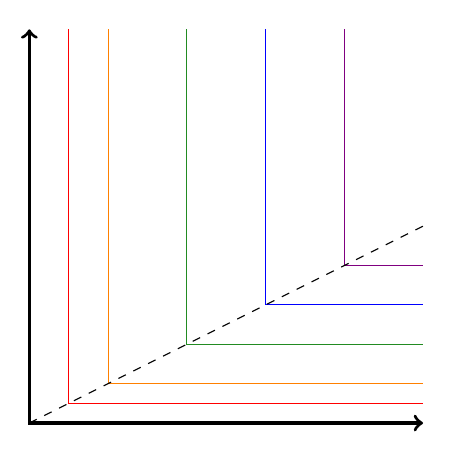
\begin{tikzpicture}[scale=0.5]
			\draw[<->,very thick] (10,0)--(0,0)--(0,10);
			\draw[orange] (2,10)--(2,1)--(10,1);
			\draw[ForestGreen] (4,10)--(4,2)--(10,2);
			\draw[blue] (6,10)--(6,3)--(10,3);
			\draw[violet] (8,10)--(8,4)--(10,4);
			\draw[red] (1,10)--(1,0.5)--(10,0.5);
			
			\draw[dashed] (0,0)--(10,5);
		\end{tikzpicture}
		\caption{Leontief Isoquants}
		\label{fig:leontief_isoquants}
	\end{figure}
	We have one good that is not produced -- $a_0 = (a_{01},a_{02},\dots,a_{0N})$. We have a labor endowment of $L$, and we call gross output $x$ and $y \le x$ net output.
	
	Call the vector $(a_{0j},\cdots,a_{Nj})$ a \blue{technique} for producing good $j$. Note that to produce some vector $x = (x_1,\dots,x_N)$, we need $Ax$ of the inputs. Then, of course, $y = x - Ax$. The question we'll face next time: Given our technology, can we produce anything?
	\end{model}
	\begin{definition}
		$A$ is \blue{productive} if $\exists x\opt \gg 0 \st x\opt \gg Ax\opt$ (equivalently: if $y = x\opt - x\opt$, $y \gg 0$).
	\end{definition}

\begin{theorem}
	If $A$ is productive, any $y \ge 0$ can be produced (\ie for any $y \ge 0, \exists x \ge 0 \st (I-A)x = y$)
\end{theorem}

\begin{proof}
\begin{lemma}
	If $A$ is productive, and $x \ge Ax$, then $x \ge 0$.
\end{lemma}
\begin{proof}
	Suppose $\exists x \not\ge 0 \st x \ge Ax$. Define $\lambda' = \inf \{\lambda : x + \lambda x\opt \ge 0\}$, where $x\opt \gg Ax\opt$ exists by productivity, and define $x' = x + \lambda'x\opt$. Then \[x+\lambda'x\opt \gg Ax + \lambda' Ax\opt = A(x + \lambda 'x\opt) \ge 0\]so $\lambda'$ is not the infimum.
\end{proof}
\begin{corollary}
	If $A$ is productive, then $I-A$ has full rank.
\end{corollary}
\begin{proof}
Suppose $(I-A)x = 0$. Then $x \ge Ax$ and $x \ge 0$. Since $(I-A)(-x) = 0$ then $-x\ge A(-x)$ and $-x \ge 0$. Thus, $x = 0$ and $(I-A)$ has a rank 0 null space.
\end{proof}

Since $I-A$ is invertible, for any $y \ge 0$ there is an $x$ such that $(I-A)x = y$, then by the Lemma $x \ge 0$.
\end{proof}


\begin{theorem}
	If $(I-A)^{-1}$ has non-negative columns and is non-singular, then $A$ is productive.
\end{theorem}
\begin{proof}
	For any $y\ge0$, $(I-A)^{-1}y \ge 0$. Since $(I-A)^{-1}$ is non-singular, it has no zero column, so every column is semi-positive. Therefore $x\opt = (I-A)^{-1}e \gg 0$, and $x\opt \gg Ax\opt$.
\end{proof}

\begin{remark}
	There are other conditions that work.
\end{remark}
\begin{theorem}
	\red{Hawkins-Simon} $A$ is productive $\Longleftrightarrow$ all leading principal minors are positive
\end{theorem}


\begin{theorem}
	If $A$ is productive, then $A^n x \to 0$ (at a geometric rate).
\end{theorem}
\begin{proof}
	Since $A$ is productive, $x\opt \gg Ax\opt$ for some $x\opt \gg 0$, and there is $\lambda \in (0,1)$ such that $\lambda x\opt \gg x\opt$. Then $Ax\opt \ll \lambda Ax\opt \ll \lambda^2x\opt$, and for all $n$ $\lambda^nx\opt \gg A^nx\opt$, so $A^nx\opt \to 0$ and $A^n \to 0$.
\end{proof}
\begin{corollary}
	If $A$ is productive, then $\lim_{n\to\infty} (I + A + A^2 + \cdots + A^n) = (I-A)^{-1}$
\end{corollary}
\begin{proof}
	$(I-A)(I + A + A^2 + \cdots + A^n) = I - A^{n+1} \to I$.
\end{proof}

Suppose that the economy is endowed with $L$ units of the (non-produced) primary good. What net output bundles can we make? To produce $y$, we need $(I-A)^{-1}y$ units of gross output, which requires $a_0 (I-A)^{-1}y$ of the primary factor. Thus, our production possibility set is \[P(L) = \{y : a_0 (I-A)^{-1}y \le L\}\]

\begin{definition}
	A \blue{price vector} $(p_0,p_1,\dots,p_N) = (p_0,p) \in \reals_+^{N+1}$ where $p_0$ is the price of the primary input and $p_i$ is the price of produced good $i$. The cost of producing one unit of good $j$ is \[c_j = p_0a_{0j} + pA^j\]and the profit from producing one unit of good $j$ is \[\pi_j = p_j - c_j = p_j - \sum_{m} p_ma_{mj}\Longrightarrow \pi = p(I-A) - p_0a_0\]
\end{definition}

\begin{definition}
	An \blue{equilibrium} is a tuple $\langle x, y, p, p_0\rangle$, such that (i) $y \le (I-A)x$, (ii) $a_0x < L \Longrightarrow p_0 = 0$, (iii) $y_m < x_m - a_m x \Longrightarrow p_m = 0$, (iv) $\pi \le 0$, (v) $\pi x = 0$, and (vi) $a_0 x \le L$.
\end{definition}
\begin{assumption}
	We set $p_0 = 1$ almost always, and deal with prices relative to labor. The exception is when we have excess labor. See condition \textnormal{(ii)} of equilibrium above.
\end{assumption}

\begin{theorem}
	If $A$ is productive and $a_0 \gg 0$, an equilibrium exists in which $y \gg 0$, $p \gg 0$, and all profits are 0.
\end{theorem}
\begin{proof}
	Per-unit profits are $\pi = p(I-A) - a_0$. If $A$ is productive, then $(I-A)$ is invertible, so take $p = (I-A)^{-1}a_0$, so $\pi =0$. Next, choose any $y$. The required labor input is $a_0 (I-A)^{-1}y$, and we can scale $y$ directly so that this equals $L$. Strict positivity of $p$ follows from the fact that $(I-A)^{-1}$ is non-negative and since it is non-singular, it has at least one non-zero element in each column. Conclusion follows from the hypothesis that $a_0 \gg 0$.
\end{proof}

\begin{remark}
	That $A$ is productive is, of course, necessary. The condition that $a_0 \gg 0$ can be relaxed, and that's very contemporary research. Specifically, we need that the product \[a_0 \Big\{ I + A + A^2 + \cdots + A^{n+1} + \cdots \Big\} \gg 0\]This would reduce the condition to $a_0 \ge 0$ and $a_0 \ne 0$, and a sufficient condition for that is the graph described by $A$ being irreducible -- \ie that if we draw a directed graph where an arrow from $i$ to $j$ means `$i$ is used in the production of $j$', that graph being irreducible implies that for sufficiently large $m$, $A^m$ is always strictly positive, which suffices to show that $(I-A)^{-1}$ is strictly positive. Note that we can reach the entirety of the indirect reach of labor with \emph{only} the first $n-1$ matrix products, where $n$ is the size of the matrix.
\end{remark}

\begin{definition}
	A \blue{convex support function} for a set $C$ is defined by the maximization problem \[v_C(q) = \max \{q \cdot x : x \in C\}\]This function is convex and homogeneous of degree 1. The \blue{concave indicator function} of a convex set $C$ is the function \[\ones_C(x) = \begin{cases} 0 & x \in C \\ -\infty & x \not\in C \end{cases}\](and the \blue{convex indicator function} is defined analogously, with $+\infty$).
\end{definition}

\begin{question}
	What does the set of convex support functions actually look like? It sits in $\cont^1$, which is a normed vector space. In fact, it is \emph{precisely} the set of continuous, homogeneous of degree 1, and convex functions, which is a convex cone! We can, in fact, even put a measure on this space and regress over it. This means that we can put a measure over all convex sets, and even prove central limit theorems and laws of large numbers over them.
\end{question}

\begin{example}
	Consider the production possibility set of our economy, where we have the production matrix $A$, the labor requirement vector $a_0$, and labor endowment $L$. The set is described by the constraints: (i) $y - (I-A)x \le 0$, (ii) $a_0x \le L$, and (iii) $x,y \ge 0$. We can define its convex support function as \[v_C(q) = \max q \cdot y \]subject to\begin{align*} y - (I-A)x &\le 0 \\ a_0x &\le L\\ x,y &\ge 0\end{align*}The dual of this problem is \[\min_{p_0,p} p_0 \cdot L \]subject to \begin{align*} p &\ge q \\-p(I-A) + p_0a_0 &\ge 0 \\p_0,p &\ge 0\end{align*}
\end{example}
\begin{remark}
	We can interpret $q$ as `world prices' in a market where only final goods are shipped.
\end{remark}
\begin{remark}
	Complimentary slackness of $p - q$ implies that $p_m > q_m \Longleftrightarrow $ we produce $0$ of good $m$, and that either we use a positive amount of good $i$ in production or we make positive profit on good $i$. Formally:
\end{remark}
\begin{corollary}
	At an optimal primal-dual quadruple $(y\opt,x\opt,p\opt,p_0\opt)$, we have that:
	\begin{enumerate}
		\item $p\opt y\opt - p\opt (I-A)x\opt = 0$, so if good $m$ is in excess supply then $p\opt_m = 0$.
		\item $p_0\opt(a_0x\opt - L) = 0$, so if labor supply is not exhausted then wage $p_0\opt = 0$.
		\item $(p\opt - q)y\opt = 0$, so if the net output of good $m$ is positive, then $p_m\opt = q_m$.
		\item $p\opt(I-A)x\opt + p_0\opt a_0x\opt = 0$, so if good $m$ is produced, profits $\pi_m = 0$.
	\end{enumerate}
\end{corollary}
\begin{remark}
	These complementary slackness conditions precisely define the equilibrium we defined above.
\end{remark}

\begin{theorem}
	If $A$ is productive and $a_0 \gg 0$, then both the primal and dual have optimal solutions. If $(x\opt,y\opt)$ solves the primal problem and $(p\opt,p_0\opt)$ solves the dual, then $(x\opt,y\opt,p\opt,p_0\opt)$ is an equilibrium.
\end{theorem}
\begin{proof}
	If $A$ is productive, the feasible set is nonempty, as the first primal inequality has at least one solution. If $a_0 \gg 0$, then it is bounded, so the primal problem attains a maximum. Conclusion follows from strong duality.
\end{proof}


\begin{model}
	\red{Activity Analysis Model of Production} We have $N$ goods, $M$ activities, $M \ge N$, a matrix $A \in \reals^{N \times M}$ where $a_{mn}$ is the amount of good $n$ needed to run activity $m$ at unit level, and $a_{0m}$ the amount of `labor' required to run activity $m$ at unit level. The only difference, besides $A$ no longer being square, is that we now have $B \in \reals^{N \times M}$, where the column $B^m$ is the output vector of goods $1,\dots,n$ from running activity $m$ at unit level.
	
	The vector $x \in \reals^m_+$ is now the vector of levels at which the different activities are run. For activity vector $x \ge 0$, the input requirements are $Ax$ and the output levels are $Bx$. 
	
	\begin{definition}
		The model is \blue{productive} if there exists $x\opt \ge 0$ such that $Bx\opt \gg Ax\opt$. The \blue{production possibility set} of the economy is \[Y = \{y \ge 0 : (B-A)x \ge y, a_0x \le L, x \ge 0\}\]
	\end{definition}
	\begin{remark}
		The general Leontief model is a special case of the Activity Analysis Model, where we assume that there is no joint production.
	\end{remark}
	\begin{definition}
		A \blue{technology} $\tau$ is a set of $N$ activities in $\{1,\dots,M\}$ such that through those activities alone every good is produced.
	\end{definition}
	The problem, therefore, is to characterize the production possibility set. Define the cost functions \begin{align*} \lambda(y) &= \min\{a_0 x: (B-A)x \ge y , x \ge 0\} \\ \lambda^\tau (y) &= \min\{a_0 x : (I-A^\tau)x \ge y, x \ge 0\}\end{align*}that gave the minimum amount of the primary factor needed to produce net output $y$ in (first) the general model and (second) the technology $\tau$. Define their respective production possibility sets as \begin{align*} P(L) &= \{y : (B-A)x \ge y , x \ge 0, a_0 x \le L\} \\ P^\tau(L) &= \{y : (I-A^\tau)x \ge y, x \ge 0, a_0x \le L\}\end{align*}Note that for any $\tau$, $P^\tau(L) \subseteq P(L)$. 
\end{model}

\begin{theorem}
	\red{Non-Substitution Theorem} There is a technology $\tau\opt$ such that for all $y \ge 0$, $\lambda(y) = \lambda^{\tau\opt}(y)$.
\end{theorem}
\begin{corollary}
	$P^{\tau\opt}(L) = P(L)$.
\end{corollary}
\begin{proof}
	First, to produce the vector $\ones$, we solve the problem \[\lambda(\ones) = \min a_0 x \st (B-A)x \ge \ones, x \ge 0\]Productivity of $A,B$ implies that the feasible set is nonempty, so this problem has a solution. This means that it has a basic optimal solution, and we call the set of its columns a technology $\tau\opt$. 
	
	Recall that for any technology $\tau$, cost is linear in $y$\[\lambda^\tau (y) = a_0 (I - A^\tau)^{-1}y\]To show that $\lambda^{\tau\opt}(y) = \lambda(y)$, it suffices to show that $\lambda^{\tau\opt}(y) \le \lambda^\tau(y)$ for any other $\tau$. 
	\begin{lemma}
		For each $\ones^m$ and for all $\tau$, $\lambda^{\tau\opt}(\ones^m) \le \lambda^\tau(\ones^m)$.
	\end{lemma}
	\begin{proof} FSOC, assume that there is a cheaper technology $\theta$ for producing $\ones^1$. Then \[\lambda(\ones) \le \lambda^\theta (\ones^1) + \sum_{m \ge 2} \lambda^{\tau\opt} (\ones^m) < \sum_{m \ge 1} \lambda^{\tau\opt} (\ones^m) = \lambda^{\tau\opt} (\ones)\]which is a contradiction. \end{proof}
	
	To conclude the proof, observe that any $y$ can be produced at minimum cost by some technology, and for any technology $\tau$, \[\lambda^\tau(y) = \sum_m y_m \lambda^\tau (\ones^m) \ge \sum_m y_m \lambda^{\tau\opt} (\ones^m) = \lambda^{\tau\opt}(y)\]
\end{proof}

\paragraph{A Brief Aside on Modeling.} A model is an abstraction of the world. A model is a set of objects and a set of relationships. In Economics, we have agents, goods, beliefs, preferences as the objects; states such as prices and capital; and relationships such as behavioral relationships (between any objects) and consistency conditions. 

\section{The Hecksher-Ohlin-Vanek Model}

\begin{model}
	\red{Leontief Version} Consider a small country with immobile capital stock $K$ and labor endowment $L$ that trades final products clothing $c$ and food $f$ on world markets at prices $p_c$ and $p_f$. The production technology for good $g$ is described by input requirement coefficients $a_{kg}$ and $a_{lg}$. Assume:
	
	\begin{assumption}\label{ass:hov_1}
		Clothing is capital-intensive, food is labor-intensive: $\frac{a_{kc}}{a_{lc}} > \frac{a_{kf}}{a_{lf}}$
	\end{assumption}
	The PPS is the set $\{(x_c,x_f) : a_{kc}x_c + a_{kf}x_f \le K, a_{lc}x_c + a_{lf}x_f \le L, x \ge 0\}$. This set is convex, and (as before) we can characterize it with its concave support function. The support function is \begin{align*} v_P(K,L) = \max_x &\; p_cx_c + p_fx_f \\ \st \qquad a_{ck}x_c + a_{fk}x_f &\le K \\ a_{cl}x_c + a_{fl}x_f &\le L \\ x &\ge 0 \end{align*}The dual is\begin{align*} v_D(p_c,p_f) = \min_{r,w}&\;rK+wL \\ \st \qquad ra_{ck} + wa_{cl} &\ge p_c \\ ra_{fk} + wa_{fl} &\ge p_f \\ r,w &\ge 0\end{align*}The complimentary slackness conditions are \begin{align*} (r\opt a_{kc} + w\opt a_{lc} - p_c)x\opt_c &= 0 \\ (r\opt a_{kf} + w\opt a_{lf} - p_f)x\opt_f &= 0 \\ r\opt(a_{kc}x\opt_c + a_{kf}x\opt_f - K) &= 0 \\ w\opt (a_{lc}x\opt_c - a_{lf}x\opt_f - L) &= 0 \end{align*}
\end{model}


We can solve this model with a few assumptions on structure. Consider:

\textbf{Case 1: $x \gg 0$.} Let $A$ denote the matrix whose rows are input requirements, $A = \matrixp{a_{kc} & a_{kf} \\ a_{lc} & a_{lf}}$. Assumption~\ref{ass:hov_1} implies that $A$ is non-singular. For a solution where $x_c,x_f \gg 0$, complementary slackness requires that \[\matrixc{r\opt & w\opt}A = \matrixc{p_c & p_f}\]meaning that price is equal to marginal cost. A positive solution will exist if and only if:
\begin{assumption}\label{ass:hov_2}
	Prices are interior: \[\frac{a_{kc}}{a_{kf}} > \frac{p_c}{p_f} > \frac{a_{lc}}{a_{lf}}\]
\end{assumption}
which is satisfiable under the assumptions. If the price ratio equalities are strict, then the dual solution $(r\opt,w\opt)$ is strictly positive. If so, complementary slackness implies that $Ax\opt = \matrixc{K&L}'$. A strictly positive solution requires that:
\begin{assumption}\label{ass:hov_3} $(K,L)$ is in the interior of the span of the columns of $A$.	
\end{assumption}


\begin{theorem}
	Suppose Assumptions~\ref{ass:hov_1}, ~\ref{ass:hov_2}, and ~\ref{ass:hov_3} hold. Then the primal and dual have unique strictly positive solutions.
\end{theorem}
\begin{remark}
	$x\opt$ maximizes GDP, and $r\opt$ and $w\opt$ are shadow prices for resource constraints. At those prices, all per-unit profits are non-positive and operating industries make 0 profits.
\end{remark}

Note that as $K$ and $L$ change within the cone, factor prices do not change.

\begin{theorem}
	\red{Factor Price Equalization Theorem} In a diversified equilibrium, for all $(K,L) \in \{y : y = Ax,x\ge 0\}$ factor prices are those prices satisfying Assumption~\ref{ass:hov_2}, which does not depend on $(K,L)$.
\end{theorem}
\begin{remark}
	Two different countries with identical technologies but different capital-labor ratios will have the same factor prices.
\end{remark}

\begin{question}
	What is the effect of an increase in the price of good $c$?
\end{question}
\begin{answer}
	Assumption~\ref{ass:hov_1} implies that the determinant of $A$ is positive, and $A^{-1}$ will have the sign pattern $\text{sgn} A^{-1} = \matrixp{+ & - \\ - & +}$. This means that an increase in $p_c$ will increase the rental rate $r$ and lower the wage rate $w$. 
\end{answer}

\begin{theorem}
	\red{Stolper-Samuelson Theorem} In a diversified equilibrium, an increase in the world price of a commodity raises the price of the factor in which it is intensive and lowers the price of the other factor.
\end{theorem}

\paragraph{The Picture.} This is entirely illustrated in Figure~\ref{fig:hov_equ}
\begin{figure}[H]
	\centering
	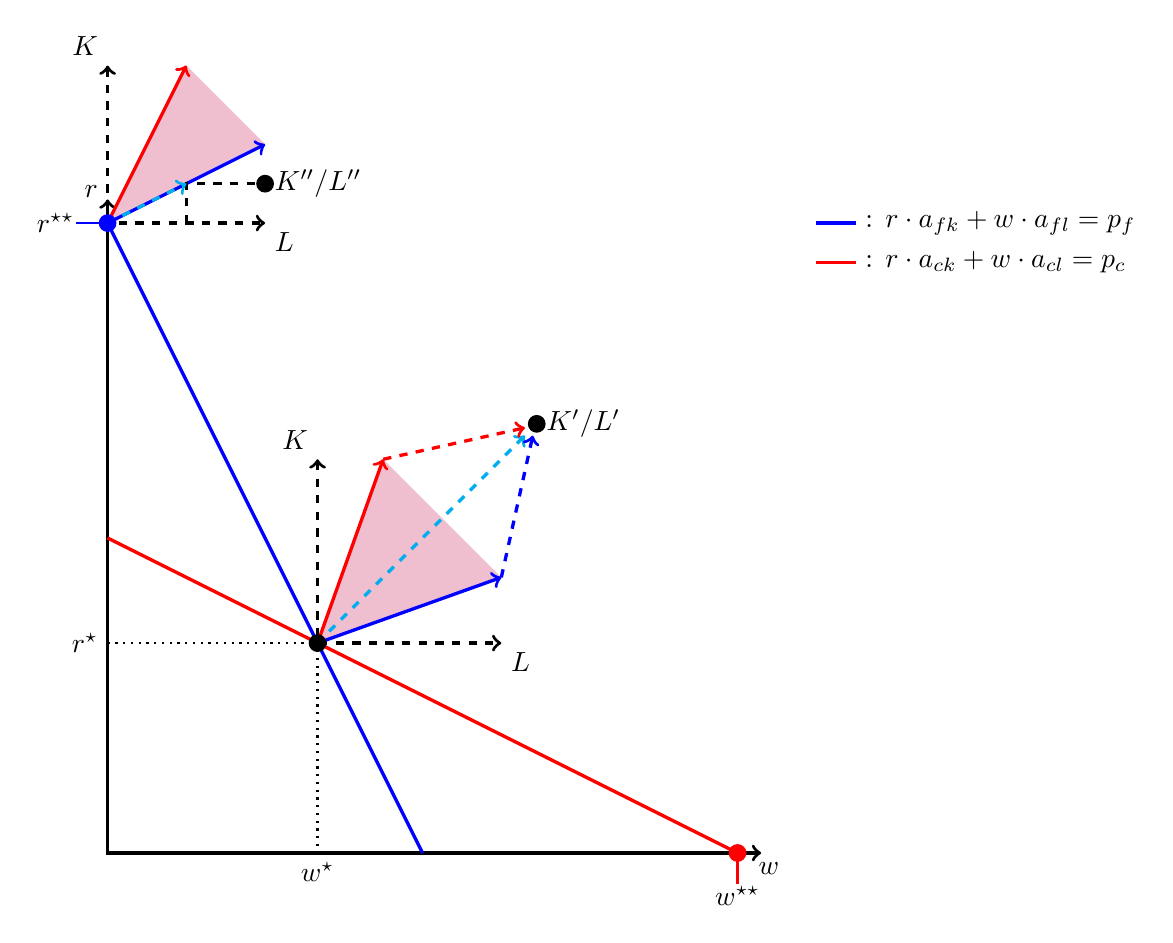
\begin{tikzpicture}
		\fill[purple, nearly transparent] (0,8)--(1,10)--(2,9)--(0,8);
		\fill[purple, nearly transparent] (2.666,2.666)--(3.5,5)--(5,3.5)--(2.666,2.666);
		\draw[very thick,<->] (0,8.3)--(0,0)--(8.3,0);
		\draw[very thick, blue] (0,8)--(4,0);
		\draw[very thick, red] (0,4)--(8,0);
		\node[left] at (0,8.4) {$r$};
		\node[below] at (8.4,0) {$w$};
		\node[left] at (0,2.666) {$r\opt$};
		\node[below] at (2.6666,0) {$w\opt$};
		\node[left] at (-0.3,8) {$r^{\star\star}$};
		\node[below] at (8,-0.3) {$w^{\star\star}$};
		\draw[red,thick] (8,0)--(8,-0.4);
		\draw[blue,thick] (0,8)--(-0.4,8);
		\draw[thick,dotted] (0,2.666)--(2.666,2.666)--(2.666,0);
		\draw[very thick, dashed,<->] (2.666,5)--(2.666,2.666)--(5,2.666);
		\draw[very thick, red, ->] (2.666,2.666)--(3.5,5);
		\draw[very thick, blue, ->] (2.666,2.666)--(5,3.5);
		\draw[very thick, dashed, cyan,->] (2.666,2.666)--(5.3,5.3);
		\draw[very thick, dashed, red, ->] (3.5,5)--(5.3,5.4);
		\draw[very thick, dashed, blue, ->] (5,3.5)--(5.4,5.3);
		\draw[very thick, dashed,<->] (0,10)--(0,8)--(2,8);
		\draw[very thick, red, ->] (0,8)--(1,10);
		\draw[very thick, blue,->] (0,8)--(2,9);
		\draw[very thick, dashed] (1,8)--(1,8.5)--(2,8.5);
		\draw[very thick, cyan,dashed,->] (0,8)--(1,8.5);
		
		\filldraw (2,8.5) circle(3pt);
		\filldraw (2.666,2.666) circle(3pt);
		\filldraw (5.45,5.45) circle(3pt);
		\filldraw[blue] (0,8) circle(3pt);
		\filldraw[red] (8,0) circle(3pt);
		\node[above left] at (2.666,5) {$K$};
		\node[below right] at (5,2.666) {$L$};
		\node[above left] at (0,10) {$K$};
		\node[below right] at (2,8) {$L$};
		\node[right] at (2,8.5) {$K'' / L''$};
		\node[right] at (5.45,5.45) {$K' / L'$};
		
		\draw[very thick, blue] (9,8)--(9.5,8);
		\node[right] at (9.5,8) {: $r\cdot a_{fk} + w\cdot a_{fl} = p_f$};
		\draw[very thick, red] (9,7.5)--(9.5,7.5);
		\node[right] at (9.5,7.5) {: $r\cdot a_{ck} + w\cdot a_{cl} = p_c$};
	\end{tikzpicture}
	\caption{A Diversified Equilibrium}
	\label{fig:hov_equ}
\end{figure}

\paragraph{The Story}
	The dot at $(w\opt,r\opt)$ is a \blue{diversified equilibrium} -- both goods are produced. The vectors are input requirements describing per-unit cost as a function of $r$ and $w$. The dual feasible factor prices are those above the \textcolor{blue}{food} and \textcolor{red}{clothing} isocost lines. The $K-L$ axes taking the intersections as their origin measure the primary factor endowment, and the \textcolor{cyan}{cyan} vector is the factor endowment. The $(K',L')$ endowment is in the cone spanned by the input requirement vectors. The requirements for the diversified equilibria are that $K',L'$ are in the cone and that the factor price vector sits on the intersection between the isocost lines for the capital- and labor-intensive industries respectively..


\paragraph{Case 2:} $x_c = 0$. Then we have that $x_f > 0$ and $ra_{fk}+wa_{fl}=p_f$. There are three subcases. There is the knife-edge case where the factor endowment vector is the same as the inputs requirement vector for some good. Equilibrium factor prices will be $(w\opt,r\opt)$, but nothing will be produced.

Alternatively, if the red isocost line lies below the blue isocost line everywhere, then only food will be produced, and one factor will be entirely exhausted. If there is excess $K$, then $r = 0$ and $w = \frac{p_f}{a_{fl}}$. If $\frac{K}{L} = \frac{a_{fl}}{a_{fk}}$, any $(r,w)$ pair on the blue isocost line is optimal. If there is excess $L$, then $w = 0$ and $r = \frac{p_f}{a_{fk}}$.

The most interesting case is if the red and blue isocost lines cross. Suppose that $K$ is in excess supply, so $a_{fk}x_f < K$. Then $r = 0$, so $w = \frac{p_f}{a_{fl}}$, so $a_{fl}x_f = L$. This solution is the $w$-intercept of the blue line. However, it's clear that this is infeasible since the solution lies below the red isocost line.

\begin{remark}
	The blue dot is a specialized equilibrium. The $(K'',L'')$ endowment is below the cone, so equilibrium is at the upper corner. Output $x_f$ is such that capital is just exhausted, and labor is in excess supply. Factor prices are $(0,r^{\star\star})$ and equilibrium factor demand is the other cyan arrow. 
\end{remark}

\paragraph{Trade.} Suppose that we now have two countries with identical technologies. Country $A$ has relatively more labor and country $B$ has relatively more capital. World prices are established in a competitive equilibrium. What is the pattern of trade?

\begin{theorem}
	\red{Rybczynski Theorem} The country with a higher ratio of capital to labor will produce relatively more of the capital-intensive good, and the country with a higher ratio of labor to capital will produce relatively more of the labor-intensive good.
\end{theorem}

Proof can be seen straightforwardly from the picture. If one country is entirely specialized, then the pattern is even stronger since they'll entirely specialize in the good they have an endowment advantage in.




\begin{model}
	\red{Smooth Version} Consider a single small country with immobile capital stock $K$ and labor endowment $L$, that trades final products $a$ and $b$ on world markets at world prices $p_a$ and $p_b$. The production technology for good $g$ is described by a production function $f_g(k,\ell)$. 
	
	\begin{assumption}\label{ass:hov_smooth}
		The production function satisfies the following:
		\begin{enumerate}
			\item $f_g \in \cont^2$
			\item $f_g$ is concave
			\item $f_g$ has constant returns to scale
			\item $f_g$ satisfies the Inada Conditions at 0: \[\lim_{k\to0} \nabla_k f_g(k,\ell') = \lim_{\ell\to0} \nabla_\ell f_g(k',\ell) = \infty \text{ for all } k',\ell' > 0\]
		\end{enumerate}
	\end{assumption}
	The profit function for industry $g$ is found by the maximization problem \[\pi_g(p_g,r,w) = \max_{k_g,\ell_g,x_g}p_gx_g - rk_g - w\ell_g \qquad \st x_g \le f_g(k_g,\ell_g)\]
	The solution to this problem gives both the output and factor demands at the output and factor market prices. Equilibrium requires that (i) outputs and factor demands are both profit maximizing, and (ii) all factor markets clear.
	
	Since production is CRS (by Assumptions~\ref{ass:hov_smooth}), cost functions are of the form $c_g(r,w)x_g$. Profit maximization requires zero profit for producers, so $p_g = c_g(r,w)$. This gives \[c_f(r,w) = p_f \qquad \text{ and } c_c(r,w) = p_c\]so Shephard's Lemma gives factor demands\[\frac{\partial c_f(r,w)}{\partial r}x_f + \frac{\partial c_c(r,w)}{\partial r}x_c = K \qquad \text{ and } \qquad \frac{\partial c_f(r,w)}{\partial \ell}x_f + \frac{\partial c_c(r,w)}{\partial \ell}x_c = L\]We have similar results to above: If $(K,L)$ is in the cone spanned by the gradients of the unit cost functions, then a diversified equilibrium would exist. Moving $(K,L)$ around inside the cone changes outputs but does not change factor prices since the first two equations are unperturbed. The gradient $\nabla c(r,w)$ is (by Shephard's Lemma) the input requirement vector. In the smooth model, the picture is Figure~\ref{fig:hov_smooth_fig}.
	
	\begin{figure}[H]
		\centering
		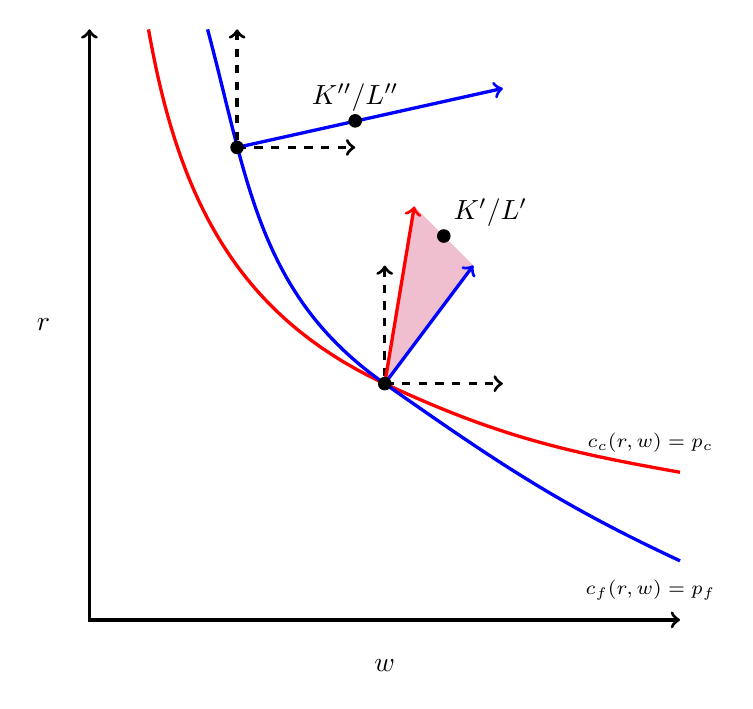
\begin{tikzpicture}[scale=0.75]
			\fill[purple, nearly transparent] (5,4)--(5.5,7)--(6.5,6)--(5,4);
			\draw[very thick, <->] (0,10)--(0,0)--(10,0);
			\node[below] at (5,-0.5) {$w$};
			\node[left] at (-0.5,5) {$r$};
			\draw[red,very thick] (1,10) to[out=-80,in=155] (5,4) to[out=-25,in=170] (10,2.5);
			\draw[blue,very thick] (2,10) to[out=-75,in=145] (5,4) to[out=-35,in=155] (10,1);
			\draw[dashed, very thick,<->] (5,6)--(5,4)--(7,4);
			\draw[dashed, very thick,<->] (2.5,10)--(2.5,8)--(4.5,8);
			\draw[blue,->,very thick] (5,4)--(6.5,6);
			\draw[red,->,very thick] (5,4)--(5.5,7);
			\draw[blue,->,very thick] (2.5,8)--(7,9);
			\filldraw (5,4) circle(3pt);
			\filldraw (2.5,8) circle(3pt);
			\filldraw (6,6.5) circle(3pt);
			\filldraw (4.5,8.45) circle(3pt);
			\node[above right] at (6,6.5) {$K'/L'$};
			\node[above] at (4.5,8.45) {$K''/L''$};
			\node at (9.5,3) {\scriptsize $c_c(r,w) = p_c$};
			\node at (9.5,0.5) {\scriptsize $c_f(r,w) = p_f$};
		\end{tikzpicture}
		\caption{The Smooth Hecksher-Ohlin-Vanek Model}
		\label{fig:hov_smooth_fig}
	\end{figure}
	\begin{remark}
		To demonstrate the Stolper-Samuelson Theorem in this model, we can apply the Implicit Function Theorem to the map \[F(r,w,p_f,p_c) = \matrixp{c_f(r,w)-p_f \\ c_c(r,w)-p_c}\]where the equilibria are the tuples for which $F(\cdot) = 0$. The Jacobian of $F$ is\[DF(\cdot) = \matrixc{D_{r,w}F(\cdot) D_{p_f,p_c}}F(\cdot) = \matrixp{\nabla c_f(\cdot) & -1 & 0 \\ \nabla c_c(\cdot) & 0 & -1}\]If we assume the hypothesis that $D_{r,w}F(\cdot)$ is non-singular, we have that \[\matrixp{\frac{\partial r}{\partial p_f} & \frac{\partial r}{\partial p_c} \\\\\frac{\partial w}{\partial p_f	} & \frac{\partial w}{\partial p_c}} = -\matrixp{\nabla c_f(\cdot)\\\nabla c_c(\cdot)} \cdot \matrixp{-1 & 0 \\ 0 & -1} = \frac{1}{\frac{\partial c_f}{\partial r}\frac{\partial c_c}{\partial w}-\frac{\partial c_c}{\partial r}\frac{\partial c_f}{\partial w}}\cdot \matrixp{\frac{\partial c_c}{\partial w} & -\frac{\partial c_f}{\partial w} \\\\-\frac{\partial c_c}{\partial r	} & \frac{\partial c_f}{\partial r}}\]The hypothesis that $c$ is capital-intensive implies that the determinant is positive, so an increase in $p_c$ lowers $w$ and raises $r$, and an increase in $p_f$ raises $w$ and lowers $r$.
	\end{remark}
\end{model}



\section{Walrasian Equilibrium}

\begin{remark}
	Think of the diamond-water paradox (appears in Smith, due to Plato). Nothing is more useful than water but it's incredibly cheap, nothing is less useful than a diamond but it's amazingly expensive. 
\end{remark}

\begin{question}
	What does the value of something actually denote? A lot of people have tried to answer this, and there's a good rundown in Larry's notes. 
\end{question}
\begin{definition}
	The \blue{marginal utility theory} (from Jevons) is that the ratio of prices is equal to the ratio of marginal utilities:
	\[\frac{MU_x}{MU_y} = \frac{p_x}{p_y}\]
\end{definition}

We can think of the different theories as a difference between classical economists, who tend to think about production and growth; and neoclassical economists, who are more interested in questions of allocation and distribution. We will think of two schools of general equilibrium theory. The \blue{Walras-Cassel} model begins with demand functions, supply functions, and a classical production model. This leads to the two-sector model and the Hecksher-Ohlin-Vanek model. This entire process is about equating supply and demand. On the other hand, \blue{Edgeworth-Pareto} use optimization -- utility maximization, profit maximization, welfare economics, etc. This leads to the modern way of conceptualizing general equilibrium theory -- especially in macroeconomics.

\paragraph{An aside on the integrability of demand.}

\begin{question}
	Why are indifference surfaces `more general' than utility functions?
\end{question}

To go from demand to utility, we use a budget balance, indirect utility, and the expenditure function:
\[v^0 = V(p^0,w^0) = U(x^M(p^0,w^0)) \quad ; \quad \mu(p,p^0,w^0) = e(p,V(p^0,m^0)) \quad ; \quad \mu(p^0,p^0,m^0) = m^0\]
where $\mu(p,p^0,w^0) = e(p,V(p^0,m^0))$ is the \blue{income compensation function}. Together, we have that\[\frac{\partial \mu(p,p^0,m^0)}{\partial p_i} = \frac{\partial e(p,V(p^0,m^0))}{\partial p_i} = x^H_i(p,v^0) = x^M_i(p,e(p,v^0)) = x^M_i(p,\mu(p,p^0,w^0))\]In summary, we define $e(p) = \mu(p,p^0,w^0)$, which solves the differential equation \[D\mu(p) = x^M_i(p,e(p)) \quad \st \quad e(p^0) = w^0\]Fix a $p\opt$ and notice that $\mu(p\opt,p,w)$ is an indirect utility function. We can invert Marshallian demand to get $\chi^m: x \to (p,w)$, and $U(c) = \mu(p\opt, \chi^m(x))$.

Can we carry out this program? If we have two or less goods, definitely! With three or more, it becomes an issue. Suppose we are given a Marshallian demand function $x^M$. Define the \blue{Slutsky substitution coefficients} \[\sigma_{ij}(p,w) = \frac{\partial x_i^M}{\partial p_j} + x^M_j \frac{\partial x_i^M}{\partial w}\]

\begin{theorem}
	Let $x^M : \reals^n_+ \times \reals_+ \to \reals^n_+$ be a Marshallian demand. If:
	\begin{enumerate}
		\item Budgets are exhausted, so $p \cdot x^M(p,w) = w$
		\item $x^M$ is differentiable throughout its domain
		\item The Slutsky coefficients are symmetric, so $\sigma_{ij} (p,w) = \sigma_{ji}(p,w)$
		\item The Slutsky matrix is negative semidefinite
		\item The magnitude of $D_wx^M$ is bounded on compact subsets of strictly positive prices
	\end{enumerate}
	then there is a utility function $U$ on the range of $x^M$ that rationalizes demand.
\end{theorem}

\paragraph{Behavioral General Equilibrium.}

Walras and Cassel posit demand functions, firm profit maximization, and search for prices that equilibrate the system. This is behavioral because individual demands are simply decision rules.

\begin{definition}
	A \blue{behavior} is a rule that maps environments into actions. In GE models, an environment for a consumer is a budget set. An environment for a firm is a price vector and a production possibility set. This is straightforward in an Arrow-Debreu economy, but is more complicated in an exchange economy.
\end{definition}

\begin{model}
	\red{Market Equilibrium from Demand} We consider an $I$-person \blue{exchange economy} with $N$ goods. Price vectors are $p \in \reals^N_+$. Each individual  $i$ is described by an endowment vector $\omega_i \in \reals^N_{+}\setminus \{0\}$ and a demand function $d_i:\reals^N_+ \times \reals^N_{+}\setminus \{0\} \to \reals^N_+$. The \blue{endowment allocation} is $\omega = \{\omega_i\}_{i\in I}$ and \blue{aggregate endowment} is $\bm{\omega} = \sum_i \omega_i$. 
	
	\begin{definition}
		\blue{Individual excess demand} is $z_i(p,\omega_i) = d_i(p,\omega_i) - \omega_i$ and \blue{aggregate excess demand} is a function $Z: \reals^N_{+}\setminus \{0\} \times \bigtimes_{i\in I} \reals^N_{+}\setminus \{0\} \to \reals^N$, where \[Z(p,\omega) = \sum_{i} d_i(p,\omega_i) - \bm{\omega}\]
		Equilibrium is \blue{market clearing}, meaning that there is no aggregate excess demand. Formally, a price vector $p \in \reals^N_{+}\setminus \{0\}$ is an \blue{equilibrium price vector} if if $Z(p,\omega) \le 0$ and $p \cdot Z(p,\omega) = 0$, so no commodity is in excess demand and if a commodity is in excess supply it has price zero.
	\end{definition}
	
	\begin{assumption}\label{ass:excess_demand}
		We make the following assumptions on the excess demand function:
		\begin{enumerate}
			\item $Z(p,\omega)$ is homogeneous of degree 0 in prices
			\item For all $p \in \reals^N_+ \setminus \{0\}$, $p \cdot Z(p,\omega) = 0$ (Walras' Law)
			\item For all $\omega$, $Z(p,\omega)$ is continuous in $p$
		\end{enumerate}
	\end{assumption}
	These can all be justified by reference to individual demand.
\end{model}

\begin{theorem}\label{thm:excess_demand_equilibrium}
	If $Z(p,\omega)$ satisfies Assumption~\ref{ass:excess_demand}, an equilibrium price vector exists.
\end{theorem}
\begin{corollary}
	If the correspondence $Z(p,\omega)$ is upper hemi-continuous in $p$ and convex-valued, then an equilibrium price vector exists.
\end{corollary}

Before we prove these, we first define the two best theorems of all time:

\begin{theorem}
	\red{Brouwer} If $C$ is a convex, compact, and non-empty set and $f: C \to C$ is a continuous function, $\exists x \in C$ such that $x = f(x)$.
\end{theorem}
\begin{theorem}
	\red{Kakutani} If $C$ is a convex, compact, and non-empty set and $F: C \rightrightarrows C$ is a nonempty, convex, and closed-valued correspondence, then $\exists x \in C$ such that $x \in F(x)$.
\end{theorem}

\begin{proof}
	(Of Theorem~\ref{thm:excess_demand_equilibrium}) The concept here is to `simulate' a price adjustment process and show that it has a fixed point. Homogeneity implies that we can restrict the price space to the unit simplex, $\Delta = \{p \in \reals^N_+ : \|p\|_1 = 1\}$. Define $f(p)$ such that $f_i(p) = \max\{-p_i,Z_i(p)\}$. Define the map $\phi: \Delta \to \Delta$ by\[\phi(p) = \frac{1}{\|p + f(p)\|_1} (p + f(p))\]To see what this does, look at \[\frac{\phi_m(p)}{\phi_n(p)} = \frac{p_m + f_m(p)}{p_n + f_n(p)}\]If $Z_m \cdot Z_n > 0$, we can't tell the relationship. If $Z_m > 0$ and $Z_n \le 0$, $f_m > 0$ and $f_n \le 0$ so $\frac{\phi_m}{\phi_n} > \frac{p_m}{p_n}$. We will use three properties of $f$: (i) $f_n > 0 \Longleftrightarrow Z_n(p,\omega) > 0$, (ii) $Z_n(p,\omega) = 0 \Longrightarrow f_n = 0$, and (iii) $p + f(p) \ge 0$.
	
	We begin by showing that $\phi$ is well-defined (\ie $\sum_n p_n + f_n(p) > 0$). Properties (i) and (ii) imply that for all goods $n$, $f_n(p)\cdot Z_n(p,\omega) \ge 0$. FSOC, assume that for some $p'$, the sum equals zero. Then by using Walras' Law, we get that \[0 = 0 \cdot Z(p',\omega) = (p' + f_n(p')) \cdot Z(p',\omega) = p'\cdot Z(p',\omega) + f_n(p') \cdot Z(p',\omega) = \sum_nf_n(p')Z_n(p',\omega)\]This and the complementary non-negativity imply that for all $n$, $f_n(p') \cdot Z_n(p',\omega) = 0$, and the contradictory supposition implies that for all $n$, $f_n(p') = -p'_n$, so each $Z_n(p,\omega) \le -p_n$. However, if $p'_n > 0$, then we have that $Z_n(p',\omega) = 0$ for all $n$, so all prices equal zero, which is a contradiction.
	
	Since $\Delta$ is compact and convex, and $f$ continuous implies that $\phi$ is continuous, we have (from Brouwer's Fixed Point Theorem) that $\phi$ has a fixed point, which we call $p\opt$. It remains to show that $p\opt$ is an equilibrium. At $p\opt$, we have that $f(p\opt) = \lambda p\opt$, where $\lambda = \|p\opt + f(p\opt)\|_1-1$. We then have that $f(p\opt) \cdot Z(p\opt,\omega) = \lambda \cdot p\opt \cdot Z(p\opt,\omega) = 0$. This and the above imply that for each $n$, $f_n(p\opt) \cdot Z_n(p\opt,\omega) = 0$. If $Z_n(p\opt,\omega) > 0$, then $f_n(p\opt) = 0$ which contradicts the assumption of positive prices. So $Z_n(p\opt,\omega) \le 0$, which together with Walras' Law implies that $p\opt$ is an equilibrium.
\end{proof}

\begin{model}
	\red{Private Ownership Economy}. A \blue{private ownership economy} is a tuple:\[\langle \{X_i,\succeq_i,\{\theta_{ij}\}_{j\in J},\omega_i\}_{i \in I},\{Y_j\}_{j \in J}\rangle\]with $I$ consumers, $J$ firms, and $N$ commodities, with consumption sets $X_i \subseteq \reals^N$, preference relations $\succeq_i$ on $X_i$, ownership shares $\theta_{ij}$, which is consumer $i$'s share of the profits of firm $j$, endowment bundles $\omega_i \in \reals^N$, and production sets $Y_j \subseteq \reals^N$. 
	
	We assume that the endowment allocation is $\omega$, the aggregate endowment is $\bm{\omega}$, the aggregate production set is $\sum_j Y_j$, that all $\theta_{ij} \ge 0$ and that $\sum_i \theta_{ij} = 1$ for all $j$. An \blue{allocation} $(x,y)$ is a specification of a \blue{consumption plan} for each consumer $i$, a vector $x_i \in X_i$, and a \blue{production plan} for each firm $j$, a vector $y_j \in Y_j$. An allocation is \blue{feasible} if and only if $\sum_i x_i = \omega + \sum_j y_j$. Following MWG, we denote the set of feasible allocations as $A \subseteq \reals^{N(I+J)}$. We will call $x$ the \blue{consumption allocation} and $y$ the \blue{production allocation} associated with the allocation $z = (x,y)$.
	
	Let $\mathcal{E} = \{\{X_i,\succeq_i,\{\theta_{ij}\}_{j\in J},\omega_i\}_{i=1}^I,\{Y_j\}_{j=1}^J\}$ denote a private ownership economy.
	
	\begin{definition}
		A \blue{competitive equilibrium} for the economy $\mathcal{E}$ is an allocation $(x\opt,y\opt)$ and a price vector $p\opt$ such that 
		\begin{enumerate}
			\item For every firm $j$, $y\opt_j$ \blue{maximizes profits} among all feasible production plans in $Y_j$, meaning that $p\opt \cdot y\opt_j \ge p\opt \cdot y_j$ for all $y_j \in Y_j$
			\item For every consumer $i$, $x\opt_j$ is \blue{preference-maximal} among  all affordable consumption plans, meaning that $x_i\opt \succeq_i x_i$ for all $x_i$ in the set \[\{x_i \in X_i : p\opt \cdot x_i \le p\opt \cdot \omega_i  + \sum_{j} \theta_{ij} \cdot p\opt \cdot y_j\opt\}\]
			\item $(x\opt,y\opt) \in A$
		\end{enumerate}
	\end{definition}
	
	\begin{theorem}
		\red{Equilibrium Existence in the Private Ownership Economy} A competitive equilibrium for $\mathcal{E}$ exists if
		\begin{enumerate}
			\item For all $I$, $X_i$ is closed, convex, and bounded from below
			\item $\succeq_i$ is locally non-satiated in $X_i$
			\item The relation $\succeq_i$ is continuous
			\item If $x'_i \succ_i x_i$, then for all $t\in (0,1)$, $tx_i' + (1-t)x_i \succ x_i$
			\item There is an $x^0_i$ in $X_i$ such that $\omega_i \gg x^0_i$
			\item For all $j$, $0 \in Y_j$
			\item The aggregate production set $Y = \sum_j Y_j$ is closed and convex
			\item $Y \cap (-Y) = \emptyset$
			\item $Y \supset \reals^N_-$
		\end{enumerate}
	\end{theorem}
\end{model}


\begin{definition}
	The \blue{Edgeworth Box} was invented in 1881, in the legendary \href{https://historyofeconomicthought.mcmaster.ca/edgeworth/mathpsychics.pdf}{Mathematical Psychics}. Edgeworth showed that: (i) barter between two people is indeterminate; (ii) all final settlements are on the contract curve; (iii) the competitive equilibrium is on the contract curve; and (iv) as the number of traders increases, the contract curve shrinks to the competitive equilibrium.
	
	When Edgeworth first drew the box, it looked like:
	\begin{figure}[H]
		\centering
		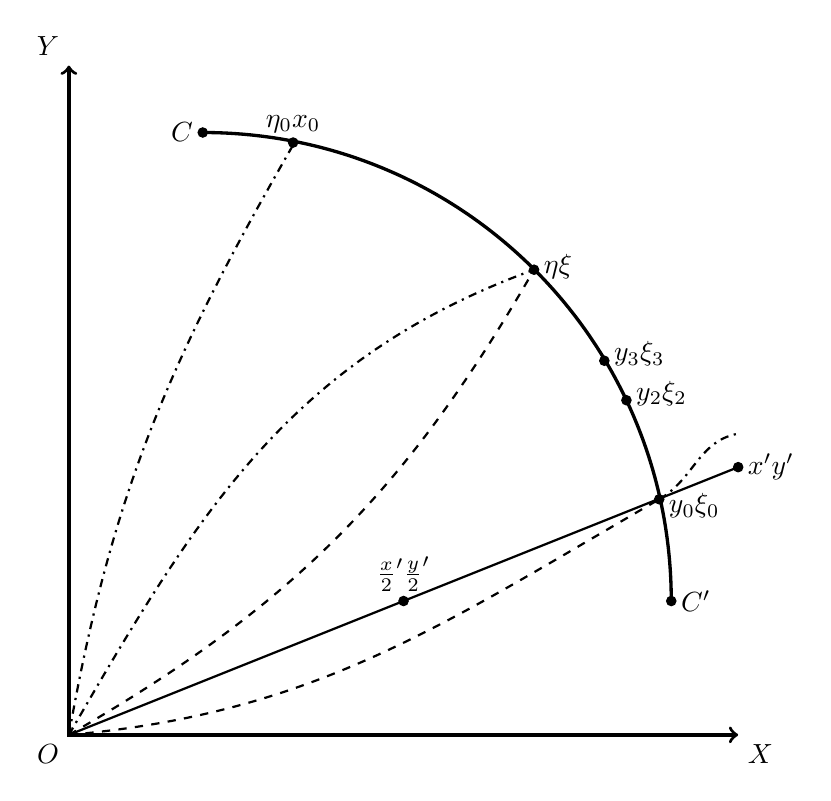
\begin{tikzpicture}[scale=0.85]
			\draw[very thick, <->] (0,10)--(0,0)--(10,0);
			\node[below right] at (10,0) {$X$};
			\node[below left] at (0,0) {$O$};
			\node[above left] at (0,10) {$Y$};
			\draw[very thick] (2,9) to[out=0,in=90] (9,2);
			\draw[thick, dash dot] (0,0) to[out=80,in=-120](3.4,8.9);
			\draw[thick, dash dot] (0,0) to[out=60,in=200] (6.95,6.95);
			\draw[thick, dashed] (0,0) to[out=30, in=240] (6.95,6.95);
			\draw[thick] (0,0)--(10,4);
			\draw[thick, dashed] (0,0) to[out=5,in=210] (8.82,3.52);
			\draw[thick, dash dot] (8.82,3.52) to[out=30,in=190] (10,4.5);
			
			\filldraw (6.95,6.95) circle(2pt);
			\filldraw (8.82,3.52) circle(2pt);
			\filldraw (5,2) circle(2pt);
			\filldraw (10,4) circle(2pt);
			\filldraw (3.35,8.85) circle(2pt);
			\filldraw (8,5.59) circle(2pt);
			\filldraw (8.33,5) circle(2pt);
			\filldraw (9,2) circle(2pt);
			\filldraw (2,9) circle(2pt);
			
			\node[left] at (2,9) {$C$};
			\node[right] at (9,2) {$C'$};
			\node[above] at (5,2) {$\frac{x}{2}'\frac{y}{2}'$};
			\node[above] at (3.35,8.85) {$\eta_0x_0$};
			\node[right] at (6.95,7) {$\eta \xi$};
			\node[right] at (8.33,5.1) {$y_2 \xi_2$};
			\node[right] at (8,5.69) {$y_3 \xi_3$};
			\node[right] at (8.82,3.42) {$y_0 \xi_0$};
			\node[right] at (10,4) {$x'y'$};
		\end{tikzpicture}
	\end{figure}
	
	We draw the Edgeworth Box for two people ($A$ and $B$) bargaining over two goods ($X$ and $Y$) like:
	\begin{figure}[H]
		\centering
		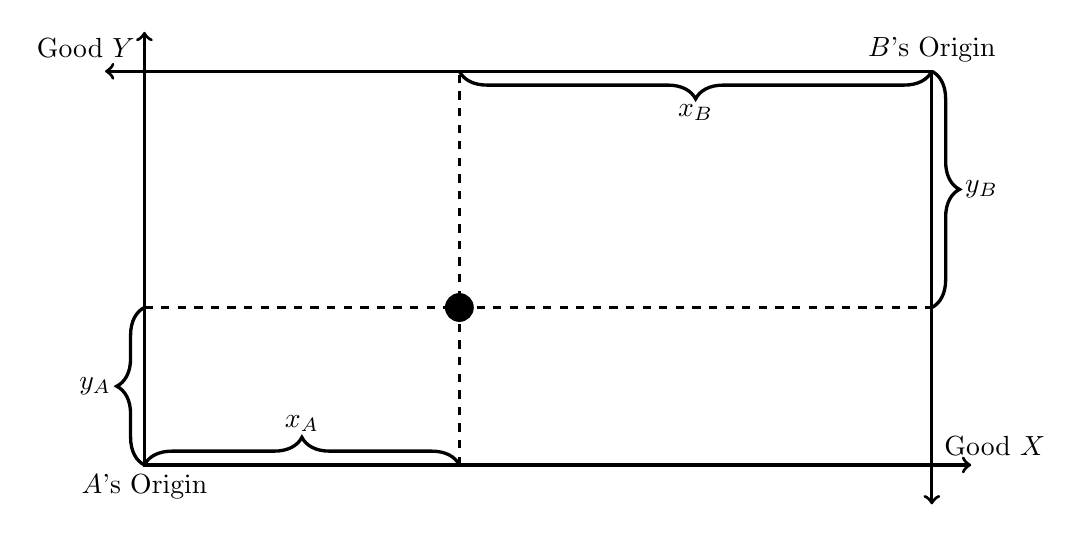
\begin{tikzpicture}
			\draw[very thick, <->] (0,5.5)--(0,0)--(10.5,0);
			\draw[very thick, <->] (-0.5,5)--(10,5)--(10,-0.5);
			\node[above] at (10,5) {$B$'s Origin};
			\node[below] at (0,0) {$A$'s Origin};
			\node[above] at (10.8,0) {Good $X$};
			\node[left] at (0,5.3) {Good $Y$};
			\draw[decorate,very thick, decoration={brace,amplitude=10pt}] (0,0)--(4,0);
			\draw[decorate, very thick, decoration={brace, amplitude=10pt}] (0,0)--(0,2);
			\draw[decorate, very thick, decoration={brace, mirror, amplitude=10pt}] (10,2)--(10,5);
			\draw[decorate, very thick, decoration={brace, mirror, amplitude=10pt}] (4,5)--(10,5);
			\node[above] at (2,0.3) {$x_A$};
			\node[left] at (-0.3,1) {$y_A$};
			\node[below] at (7,4.7) {$x_B$};
			\node[right] at (10.3,3.5) {$y_B$};
			\draw[dashed, very thick] (0,2)--(10,2);
			\draw[dashed, very thick] (4,0)--(4,5);
			\filldraw (4,2) circle(5pt);
		\end{tikzpicture}
	\end{figure}
	
	We can also represent the contract curve and the competitive equilibrium in this box, as in Figure~\ref{fig:edgeworth_examples}.
	
	\begin{figure}[H]
		\centering
		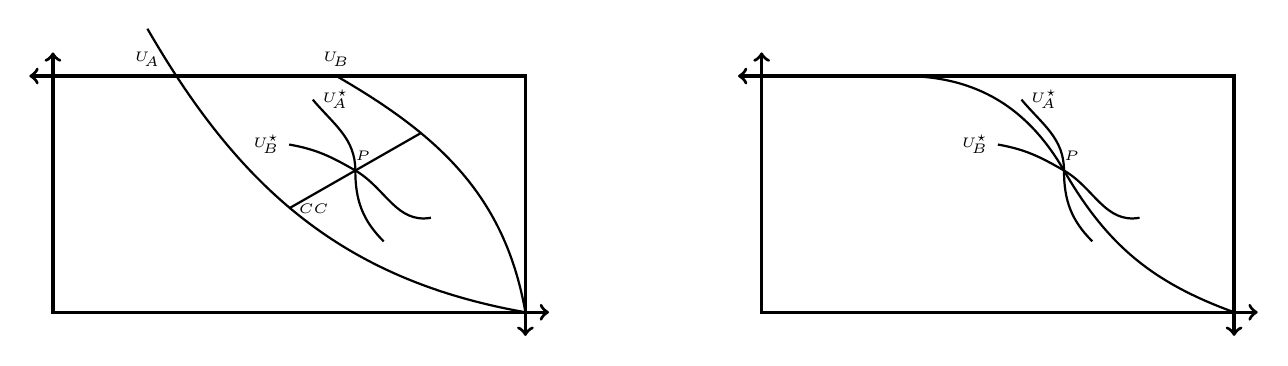
\begin{tikzpicture}[scale=0.6]
			\draw[very thick, <->] (0,5.5)--(0,0)--(10.5,0);
			\draw[very thick, <->] (-0.5,5)--(10,5)--(10,-0.5);
			% Contract curve paths
			\draw[thick] (2,6) to[out=-60,in=170] (10,0);
			\draw[thick] (6,5) to[out=-30,in=100] (10,0);
			\draw[thick] (5,2.2)--(7.8,3.8);
			\draw[thick] (5.5,4.5) to[out=-50,in=90] (6.4,3) to[out=-90] (7,1.5);
			\draw[thick] (5,3.55) to[out=-10,in=150] (6.4,3) to[out=-30,in=190] (8,2);
			\node[right] at (5.5,4.5) {\tiny $U_{\!A}\opt$};
			\node[left] at (5,3.55) {\tiny $U_{\!B}\opt$};
			\node[above] at (6.56,3) {\tiny $P$};
			\node[right] at (5,2.2) {\tiny $CC$};
			\node[above] at (2,5) {\tiny $U_{\!A}$};
			\node[above] at (6,5) {\tiny $U_{\!B}$};
			
			\draw[very thick, <->] (15,5.5)--(15,0)--(25.5,0);
			\draw[very thick, <->] (14.5,5)--(25,5)--(25,-0.5);
			\draw[thick] (20.5,4.5) to[out=-50,in=90] (21.4,3) to[out=-90] (22,1.5);
			\draw[thick] (20,3.55) to[out=-10,in=150] (21.4,3) to[out=-30,in=190] (23,2);
			\draw[thick] (18,5) to[out=0,in=120] (21.4,3) to[out=-60,in=160] (25,0);
			\node[right] at (20.5,4.5) {\tiny $U_{\!A}\opt$};
			\node[left] at (20,3.55) {\tiny $U_{\!B}\opt$};
			\node[above] at (21.56,3) {\tiny $P$};
		\end{tikzpicture}
		\caption{The Contract Curve (left) and the Competitive Equilibrium (right)}
		\label{fig:edgeworth_examples}
	\end{figure}
\end{definition}

\begin{model}
	\red{Walras Production Model} Individuals own factors and consume goods. Goods are made from factors with a fixed-coefficient technology. We have $x_j$ production of good $j$, $p_j$ price of good $j$, and $f_j(p,w)$ demand for good $j$, for $j = 1,\dots,N$. We also have $w_i$ rate of return for factor $i$, $a_{ij}$ quantity of factor $i$ needed per unit of good $j$ output, and $g_i(p,w)$ supply of factor $i$, for $i=1,\dots,M$. An \blue{equilibrium} is a triple $(p\opt,w\opt,x\opt) \in \reals^N_+ \times \reals^M_+ \times \reals^N_+$ such that: (i) each $f_n(p,w) \le x_n$ and strict inequality implies that $p_n\opt = 0$; (ii) each $(Ax)_m \le 0$ and strict inequality implies that $w\opt_m = 0$; and (iii) each $p\opt_n \le (w\opt A)_n$ and strict inequality implies that $x_n\opt = 0$. 
	
	\begin{assumption}\label{ass:walras_prod}
		We assume that:
		\begin{enumerate}
			\item $f(p,w)$, $g(p,w)$ are continuous, non-negative, and homogeneous of degree 0
			\item $p \cdot f(p,w) - w \cdot g(p,w) = 0$ (\blue{Walras' Law})
			\item $A$ has no zero columns
			\item $g(p,0) = 0$ for all $p$
		\end{enumerate}
	\end{assumption}
	
	Let $\Delta$ be the unit simplex in $\reals^{2N+M}_+$. Define $Z : \Delta \to \reals^{2N+M}$ by \[Z(p,w,x) = \matrixp{f(p,w)-x \\ Ax - g(p,w) \\p - A^Tw}\]It follows from Walras' Law that $(p,w,x)Z(p,w,x) = 0$ for all $(p,w,x) \in \Delta$. From the proof of Theorem~\ref{thm:excess_demand_equilibrium} it follows that there exists $(p\opt,w\opt,x\opt)$ such that $Z(p\opt,w\opt,x\opt)\le0$. Also $(p\opt,w\opt) \ne 0$ because Assumption~\ref{ass:walras_prod} part 4 would imply that then $x\opt = 0$. Together with Walras' Law, this implies the complimentary slackness conditions. The key technical idea is:
	
	\begin{lemma}
		\red{Gale-Kuhn-Nikaido-Debreu} If some continuous function $f$ maps the unit simplex in some Euclidean space into that space, and if for all $x$ in the simplex $x \cdot f(x) = 0$, then there is $x\opt$ in the simplex such that $f(x\opt) \le 0$.
	\end{lemma}
\end{model}


\section{Welfare}

\begin{definition}
	A \blue{competitive equilibrium with transfers} for the economy $\mathcal{E}$ is an allocation $(x\opt,y\opt)$, a price vector $p\opt$, and an assignment of wealths $(w_1\opt,\dots,w_I\opt)$ to consumers such that
	\begin{enumerate}
		\item For every firm $m$, $y_m\opt$ maximizes profits among all feasible production plans in $Y_m$:\[p\opt \cdot y\opt_m \ge p\opt \cdot y_m \text{ for all } y_m \in Y_m\]
		\item For every consumer $n$, $x_n\opt$ is preference-maximal among all affordable consumption plans; that is $x_n\opt \succeq_n x_n$ for all $x_n$ in the set \[\{x_n : x_n \in X_n \text{ and } p\opt \cdot x_n \le w_n\opt\}\]
		\item $(x\opt,y\opt) \in A$
		\item $\sum_n w_n\opt = \sum_n p\opt \cdot \omega + \sum_m p\opt \cdot y\opt_m$
	\end{enumerate}
\end{definition}

\begin{definition}
	Economists are mainly concerned with the \blue{Pareto order}. A consumption plan $x$ is \blue{Pareto-better-than} consumption plan $x'$, written $x \succ_P x'$, if for all $n$, $x_n \succeq_n x_n'$, and for some consumer $k$, $x_k \succ_k x'_k$. An allocation $z = (x,y)$ is \blue{Pareto optimal} if it is feasible and if for no other feasible consumption plan $z' = (x',y')$ is it true that $z' \succ_P z$.
\end{definition}
\begin{remark}
	How do we know that an optimum exists? 
\end{remark}
In exchange economies, this is fairly easy, as the set of feasible allocations is obviously compact, so as long as preferences are continuous we have it immediately. When we introduce production, showing that the set of feasible allocations is compact is not so straightforward. The following argument comes from \href{http://digamo.free.fr/debreu59.pdf}{Debreu (1959)}.

\begin{theorem}
	The private ownership economy $\mathcal{E}$ has an optimum if
	\begin{enumerate}
		\item For all $n$, $X_n$ is closed and bounded from below and $\omega_n \in X_n$
		\item Each $Y_m$ is closed, convex, and contains 0
		\item $Y \cap \reals^n_+ = \{0\}$ and $Y \cap -Y = \{0\}$
		\item For every $x_n' \in X_n$, the set $\{x_n \in X_n : x_n \succeq_n x'_n\}$ is closed
	\end{enumerate}
\end{theorem}
\begin{proof}
	Define $Y = \sum_m Y_m$. Consider the economy $\mathcal{E}'$ formed by replacing each $Y_m$ with their sum $Y$. Let $A'$ be the set of attainable states of $\mathcal{E}'$. Using the same preferences $\{\succeq_n\}$ as $\mathcal{E}$, and summing them, we get the continuous representation $\succeq'$, which admits the utility function $u'$, representing an order over $A'$ in $\reals^m$. However, we have that $A'$ is closed and bounded, taking condition (4) in each direction, and $A'$ is nonempty, so it's nontrivially compact and $u'$ attains a maximum. Conclusion follows by disaggregating $u'$ and $a\opt \in A'$ into their component parts.
\end{proof}

We can now move to the actual welfare theorems. First:

\begin{definition}
	Recall that a preference order $\succeq_n$ is \blue{locally non-satiated} at $x_n\opt$ if in every open neighborhood of $x_n\opt$ there is an $x_n' \succ_n x_n\opt$.
\end{definition}


\begin{theorem}\label{thm:first_welfare_theorem}
	\red{First Welfare Theorem} Let $\mathcal{E}$ be a private ownership economy with an equilibrium $(p\opt,x\opt,y\opt)$. Suppose for all $n$, $\succeq_n$ is everywhere locally non-satiated. Then $(x\opt,y\opt)$ is a Pareto-optimal allocation.
\end{theorem}
\begin{remark}
	A failure of the First Welfare Theorem is that the proof requires that in every equilibrium, any consumption bundle that is better for some $n$ costs more. Actually, it requires more -- it requires that any bundle that is at least as good costs at least as much. Thus, a thick indifference curve can break it, and that's not such an absurd assumption.
\end{remark}


\begin{proof}
	First, a useful Lemma:
	\begin{lemma}\label{lem:lns_prices}
		If $\succeq_n$ is locally non-satiated at bundle $x_n'$ and if $x_n' \succeq_n x_n\opt$, where $x\opt_n$ is preference-maximal on the set $\{x_n \in X_n : p\cdot x_n \le p \cdot x_n\opt\}$, then $p \cdot x_n' \ge p \cdot x_n\opt$.
	\end{lemma}
	\begin{proof}
		Since $\succeq_n$ is locally non-satiated at $x_n'$, there exists a sequence of consumption bundles $x_n^k$ with limit $x_n'$ such that $x_n^k \succ_n x_n'$ for all $k$. By transitivity, $x_n^k \succ_n x_n\opt$, and so by preference maximality $p \cdot x_n^k > p \cdot x_n\opt$ for all $k$. Taking limits, we get that $p \cdot x_n' \ge p \cdot x_n\opt$.
	\end{proof}
	
	Suppose FSOC that there is some feasible bundle $(x',y')$ such that $(x',y') \succ_P (c\opt,y\opt)$. Then for all $n$, $x_n' \succeq_n x_n\opt$, and for someone this ranking is strict. Then from Lemma~\ref	{lem:lns_prices}, we have that $p\opt \cdot x_n' \ge p\opt \cdot x_n\opt$ for all $n$, with the inequality strict for some. Furthermore, for each firm $j$ we have that $p\opt \cdot y_m' \le p\opt \cdot y_m\opt$ since each firm maximizes profit in equilibrium. Thus,\[p\opt \cdot \omega = p\opt \sum_n x_n\opt - p\opt \sum_m y_m\opt < p\opt \sum_n x_n' - p\opt \sum_m y_m'\]The equality follows from feasibility of the equilibrium allocation, the inequality follows from the above conditions, and thus we have that $(x',y')$ is not feasible, leading to a contradiction.
\end{proof}


\begin{definition}
	Let $P(x_n) = \{x_n' \in X_n : x_n' \succ_n x_n\}$ be the \blue{better-than set} and let $R(x_n) = \{x_n' \in X_n : x_n' \succeq_n x_n\}$ be the \blue{no-worse-than set}. A \blue{quasi-equilibrium} for the economy $\mathcal{E}$ is an allocation $(x\opt,y\opt)$ and a price vector $p\opt$ such that 
	\begin{enumerate}
		\item For every firm $m$, $y\opt_m$ maximizes profits among all feasible production plans in $Y_m$: \[p\opt \cdot y_m\opt \ge p\opt y_m' \forall y_m \in Y_m\]
		\item For every consumer $n$, $x_n\opt$ is expenditure-minimal on $R(x_n\opt)$, meaning that $p\opt \cdot x_n\opt \le p\opt \cdot x_n \forall x_n \in R(x_n\opt)$
		\item $(x\opt,y\opt) \in A$
	\end{enumerate}
	A quasi-equilibrium is sometimes called a \blue{compensated equilibrium}.
\end{definition}

\begin{theorem}\label{thm:second_welfare_theorem}
	\red{Second Welfare Theorem} Let $(x\opt,y\opt)$ be a Pareto optimal allocation for a private ownership economy $\mathcal{E}$ with the properties that
	\begin{enumerate}
		\item For all $n$, $X_n$ is convex
		\item The sets $R(x_n\opt)$ are convex
		\item For some consumer $k$, $P(x_k\opt)$ is convex and $\succeq_k$ is locally non-satiated at $x\opt_k$
		\item $Y$ is convex
	\end{enumerate}
	Then there is $p\opt$ such that $(x\opt,y\opt,p\opt)$ is a quasi-equilibrium for $\mathcal{E}$.
\end{theorem}
\begin{proof}
	Define the set $G = \sum_{n\ne k} R(x_n\opt) + P(x_k\opt) - Y$. This set is convex and $\omega$ is not in $G$ because the allocation is Pareto optimal. This, there is a vector $p\opt$ such that $p\opt \cdot \omega \le p\opt \cdot g$ for all $g \in G$. Since consumer $k$ has preferences that are locally non-satiated, there is a sequence of consumption plans $x_k^i$ such that as $i \to \infty$, $x_k^i \to x_k\opt$, where $x_k^i \succ_k x_k\opt$ for all $i$. Then for all $n$ the vector \[g^i = \sum_{n\ne k} x_n\opt + x_k^i - \sum_m y_m\opt\]is in $G$, and the sequence $g^i$ converges to\[\omega = \sum_{n\ne k} x_n\opt + x_k\opt - \sum_m y_m\opt\]Thus, $\omega \in \partial G$ and $\inf\{p\opt \cdot g : g \in G\} = p\opt \cdot \omega$. Now, we will show that $(x\opt,y\opt,p\opt)$ is a quasi-equilibrium. Intuitively, we need that everything at least as good costs at least as much, and profit maximization. For $n \ne k$ and for any $x_n' \in R(x_n\opt)$, let \begin{align*} g_n^i &= \sum_{j\ne n,k} x_j\opt + x_n' + x_k^i - \sum_m y_m\opt \\\omega &= \sum_{j\ne n,k} x_j\opt + x_n\opt + x_k\opt - \sum_m y_m\opt\end{align*}Each $g^i_n \in G$, so $p\opt \cdot g^i_n \ge p\opt \cdot \omega$. Taking limits and subtracting, $p\opt \cdot x_n' \ge p\opt \cdot x_n\opt$. We can do the same by taking any $y_m' \in Y_m$, and seeing that $-p\opt \cdot y_m\opt \ge -p\opt \cdot y_m'$ for all $y'_m \in Y_m$, meaning that $y_m\opt$ is profit-maximizing. For consumer $k$, we can see directly by subtraction that for all $x'_k \succ_k x_k\opt$, $p\opt \cdot x_k' \ge p\opt \cdot x_k\opt$, and the conclusion for all $x'_k \succeq_k x_k\opt$ follows from local non-satiation.
\end{proof}

\begin{question}
	When is a quasi-equilibrium not a competitive equilibrium? 
\end{question}
\begin{remark}
	The existence of $x_i'$ is often referred to as the \blue{cheaper point assumption}. The following figure illustrates what can go wrong if the cheaper point does not exist:
	\begin{figure}[H]
		\centering
		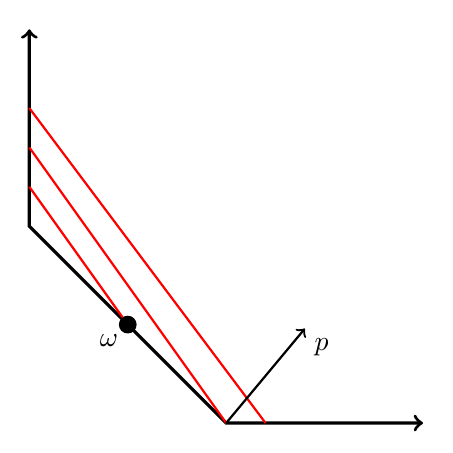
\begin{tikzpicture}
			\draw[very thick, <->] (0,5)--(0,2.5)--(2.5,0)--(5,0);
			
			\node[below left] at (1.25,1.25) {$\omega$};
			
			\draw[red,thick] (1.25,1.25) --(0,3);
			\draw[red,thick] (0,3.5)--(2.5,0);
			\draw[red,thick] (0,4)--(3,0);
			\draw[black, thick, ->] (2.5,0)--(3.5,1.2);
			\node[below right] at (3.5,1.2) {$p$};
			
			
			\filldraw[black] (1.25,1.25) circle(3pt);
		\end{tikzpicture}
	\end{figure}
	The consumption set is $\reals^2_+$ from which the open triangle with vertices at $e_1$, $e_2$, and $0$ is removed. Prices and wealth are such that the budget set is the lower 45 degree line. The red lines are indifference curves, and the indicated consumption bundle $\omega$ is expenditure maximizing on its `no worse than' set but is not preference maximal on the budget set.
\end{remark}

\begin{remark}
	To move from quasi-equilibrium to competitive equilibrium, we need expenditure minimization to imply utility maximization, meaning that if $x_n\opt$ minimizes expenditure at price $p\opt$ on the set $P(x_n\opt)$, the $x\opt$ is preference maximal on the set $\{z : p\opt \cdot z \le p\opt \cdot x_n\opt\}$.
\end{remark}

\begin{lemma}\label{lem:cheaper_point}
	\red{Cheaper Point Lemma} Suppose that at price $p$, $x_n'$ minimizes expenditure on $R(x_n')$. Suppose that $P(x_n')$ is open and that there is an $x_n^0 \in X_n$ such that $p \cdot x_n^0 < p \cdot x_n'$. Then $x_n'$ is preference maximal on the set $\{x''_n \in X_n : p \cdot x''_n \le p \cdot x_n'\}$. 
\end{lemma}
\begin{proof}
	If $x_n'$ is expenditure minimizing on $R(x_n')$, then $x_n'' \succ_n x_n'$ implies that $p \cdot x_n'' \ge p \cdot x_n'$. We must show that this inequality is strict. Suppose FSOC that $p \cdot x_n'' = p \cdot x_n'$. Since $p \cdot x_n^0 < p \cdot x_n'$, we have that $x''_n \succ_n x'_n \succ_n x_n^0$. For all $t \in (0,1)$, \[p \cdot (t \cdot x''_n + (1-t) \cdot x_n^0) < p \cdot x_n'\]and for $t$ sufficiently close to 1, $(t \cdot x''_n + (1-t) \cdot x_n^0) \succ_n x_n'$, which contradicts expenditure minimization. 
\end{proof}

\begin{theorem}
	\red{From Quasi- to Competitive Equilibrium} Suppose that $(x\opt,y\opt,p\opt)$ is a quasi-equilibrium for a competitive ownership economy $\mathcal{E}$. Suppose that for all consumers $n$ and for all $x_n \in X_n$, the set $\succ_n(x_n)$ is open. If each $w_n\opt = p\opt \cdot x_n\opt \ge 0$, then $(x\opt,y\opt,p\opt,w\opt)$ is a competitive equilibrium with transfers. 
\end{theorem}
\begin{proof}
	Immediate consequence of the definition of a quasi-equilibrium and the \href{lem:cheaper_point}{Cheaper Point Lemma}.
\end{proof}
\begin{remark}
	The cheaper point assumption is automatically satisfied for interior optima. What about boundary optima?
\end{remark}

\paragraph{Lange's Approach} If $x\opt$ is an interior (strictly) Pareto optimal allocation, then there is no reallocation that can increase the utility of any consumer without decreasing the utility of anyone else. Let $u_n(x_n\opt) = u_n\opt$. Then $x\opt$ solves the optimization problem on $\bigtimes_n X_n$:
\begin{align*}
	PO(x\opt) \;:\; \max &\;u_i(x_i) \\\st \quad u_n(x_n) &\ge u_n\opt \\\sum_n x_n &= \sum_n x_n\opt
\end{align*}
Assume that the $u_n(\cdot)$ are strictly increasing and $\cont^1$, and we can assume the weak inequalities hold with equality. For simplicity, we'll consider an interior allocation. The first order conditions are
\begin{align*}
	Du_1(x_1) &= \lambda \\ \nu_n Du_1(x_1) &= \lambda \forall n \ne 1
\end{align*}
for some $\lambda \in \reals^L$ and $\nu_n \in \reals$, together with the constraints. Strict monotonicity will imply that $\lambda,\nu \gg 0$. From this, the usual equality constraints for marginal rates of substitution follow. These conditions, along with the constraints are necessary for an allocation to be Pareto optimal. If we assume the $u_n$ are quasiconcave, these are also sufficient.

Now suppose an allocation $x_1',\dots,x_I'$ is a competitive equilibrium at price vector $p$. Then $\sum_n x_n' = \sum_n \omega_n$, and for each $n$ the bundle $x_n'$ solves the maximization problem \[CE_n(\omega_n) \;:\; \max u_n(x_n) \qquad \st \qquad p \cdot x_n \le p \cdot \omega_n\]Again, we can take the inequality to be an equality. The first order conditions include $Du_n(x\opt_n) = \eta_n \cdot p$. Again, these conditions are necessary, and suffice if $u_n(\cdot)$ are quasiconcave.

Suppose that the $u_n(\cdot)$ are quasiconcave. The welfare theorems in these terms are:
\begin{theorem}
	\red{FWT (Lange)} If for all $n$ and $x_n\opt$, $\eta_n$ solve the first order conditions for $CE_n(x_n\opt)$ with prices $p$, then $x\opt$ and multipliers $\lambda = \eta_1 \cdot p$ and $\nu_n = \eta_1 / \eta_n$ solve the $PO(x\opt)$ first order conditions.
\end{theorem}
\begin{theorem}
	\red{SWT (Lange)} If $x\opt$, $\nu$, and $\lambda$ solve $PO(x\opt)$, then taking $\nu_1 = 1$, $x\opt$ and the multipliers $\eta_n = 1/\nu_n$ and $p = \lambda$ solve all of the $CE_n(x_n\opt)$ first order conditions. 
\end{theorem}
Due to quasiconcavity of the $u_n(\cdot)$, the first-order conditions are sufficient as well, and so for every interior Pareto optimal allocation there is a price that makes it a no-trade competitive equilibrium; and every competitive allocation is Pareto optimal.



\section{Transferable Utility Matching}

\begin{model}
	The market contains \blue{workers} and \blue{firms}. Workers and firms are \blue{matched} together, one-to-one. Utility is \blue{transferable} among workers and firms, and if a match is formed it will generate \blue{surplus}. We ask if (i) we can characterize optimal matches; (ii) we can decentralize them in some sort of market; (iii) allocate the surplus between firms and workers; and (iv) implement the market solution with some mechanism. The classic article is \href{https://link.springer.com/article/10.1007/BF01753437}{Shapley \& Shubik (1971)}. 
	
	Formally, we have $\mathcal{L}$ workers and $\mathcal{F}$ firms, where $\mathcal{X} = \matrixc{x}_{\ell f}$ is the matrix denoting whether $\ell$ is matched to $f$ (1) or not (0), $v_{\ell f}$ is the surplus from matching $\ell$ to $f$, and $\pi_f$ and $w_\ell$ are the profit of firm $f$ and the wage to worker $\ell$ respectively. 
	
	A matching is \blue{optimal} if and only if it solves the following maximization problem of total surplus:
	\begin{align*}
		v(\mathcal{L} \cup \mathcal{F}) = \max_{\ell,f} &\; v \cdot x \\ \st \qquad \sum_f x_{\ell f} &\le 1 \forall \ell \in \mathcal{L}\\\sum_\ell x_{\ell f} &\le 1 \forall f \in \mathcal{F} \\ x_{\ell f} &\in \{0,1\} \forall \ell \in \mathcal{L},f \in \mathcal{F}
	\end{align*}
	\begin{example}
		Consider the following example:
		\begin{figure}[H]
			\centering
			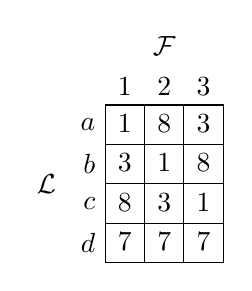
\begin{tikzpicture}[scale=0.5]
				\draw (0,0)--(3,0)--(3,-4)--(0,-4)--(0,0);
				\draw (0,-1)--(3,-1);
				\draw (0,-2)--(3,-2);
				\draw (0,-3)--(3,-3);
				\draw (1,0)--(1,-4);
				\draw (2,0)--(2,-4);
				
				\node[below] at (0.5,0) {$1$};
				\node[below] at (1.5,0) {$8$};
				\node[below] at (2.5,0) {$3$};
				\node[below] at (0.5,-1) {$3$};
				\node[below] at (1.5,-1) {$1$};
				\node[below] at (2.5,-1) {$8$};
				\node[below] at (0.5,-2) {$8$};
				\node[below] at (1.5,-2) {$3$};
				\node[below] at (2.5,-2) {$1$};
				\node[below] at (0.5,-3) {$7$};
				\node[below] at (1.5,-3) {$7$};
				\node[below] at (2.5,-3) {$7$};
				\node[above] at (0.5,0) {$1$};
				\node[above] at (1.5,0) {$2$};
				\node[above] at (2.5,0) {$3$};
				\node[left] at (0,-0.5) {$a$};
				\node[left] at (0,-1.5) {$b$};
				\node[left] at (0,-2.5) {$c$};
				\node[left] at (0,-3.5) {$d$};
				\node[above] at (1.5,1) {$\mathcal{F}$};
				\node[left] at (-1,-2) {$\mathcal{L}$};
			\end{tikzpicture}
		\end{figure}
		The optimal match is clearly $a \leftrightarrow 2$, $b \leftrightarrow 3$, $c \leftrightarrow 1$, and $d \leftrightarrow \emptyset$. Note that everyone's wage is 1 who matches -- even though the unemployed worker makes nothing, even just by existing and having productivity of 7 they constrain everyone else's wages.
	\end{example}
	
	A \blue{payoff} is a vector $(w_\ell,\pi_f)_{\ell,f \in \mathcal{L} \cup \mathcal{F}} \ge 0$, and an \blue{allocation} is a matching-payoff pair $(x,w,\pi)$ such that:
	\begin{enumerate}
		\item If $x_{\ell f} = 1$, then $w_\ell + \pi_f = v_{\ell f}$
		\item If $x_{\ell f} = 0$ for all $f$, then $w_\ell = 0$
		\item If $x_{\ell f} = 0$ for all $\ell$, then $\pi_f = 0$
	\end{enumerate}
	Finally, an allocation $(x,w,\pi)$ is \blue{stable} if no currently unmatched worker-firm pair could increase their total surplus by matching to each other, meaning that if $x_{\ell f} = 0$, then $w_\ell + \pi_f \ge v_{\ell f}$.
	
	We could relax the above non-linear program to 
	\begin{align*}
		v_P(\mathcal{L} \cup \mathcal{F}) = \max_{\ell,f} &\; v \cdot x \\ \st \qquad \sum_f x_{\ell f} &\le 1 \forall \ell \in \mathcal{L}\\\sum_\ell x_{\ell f} &\le 1 \forall f \in \mathcal{F} \\ x_{\ell f} &\ge 0 \forall \ell \in \mathcal{L},f \in \mathcal{F}
	\end{align*}
	The set $C$ of all vectors satisfying these constraints is a convex polytope, the \blue{fractional matchings}.
	
	\begin{theorem}
		\red{Birkhoff--von Neumann} $x$ is a vertex of $C$ if and only if for all $\ell,f$ $x_{\ell f} \in \{0,1\}$.
	\end{theorem}
	Thus, using the basic optimal solutions, it suffices to solve the true linear program and find an optimal matching. Formally:
	\begin{corollary}
		$x\opt$ is an optimal matching if and only if it is a basic optimal solution to the linear program.
	\end{corollary}
	The dual is, of course,
	\begin{align*}
		v_D(\mathcal{L} \cup \mathcal{F}) = \min_{\pi,w} &\; \sum_{\ell,f} w_\ell + \pi_f \\ \st\qquad w_\ell + \pi_f &\ge v_{\ell f} \forall \ell \in \mathcal{L},f \in \mathcal{F} \\ w_\ell,\pi_f &\ge 0 \forall \ell \in \mathcal{L},f \in \mathcal{F} 
	\end{align*}
	The dual has a solution $(w\opt,\pi\opt)$, where $\sum_{\ell f} w\opt_\ell + \pi\opt_f = \sum_{\ell f} v_{\ell f} x\opt_{\ell f}$. If $x\opt_{\ell f} = 1$, then $w_\ell\opt + \pi_f\opt = v_{\ell f}$. If $\ell \in \mathcal{L}$ is unmatched, then $w\opt_\ell = 0$, and if $f \in \mathcal{F}$ is unmatched, then $\pi\opt_f = 0$. We immediately get that:
	\begin{theorem}
		$(x\opt,w\opt,\pi\opt)$ is a stable allocation if and only if $x\opt$ is an optimal matching and $(w\opt,\pi\opt)$ solves the dual linear program.
	\end{theorem} 
\end{model}

\begin{example}
	Consider the surplus matrix 
	\begin{figure}[H]
			\centering
			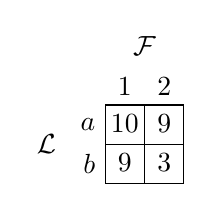
\begin{tikzpicture}[scale=0.5]
				\draw (0,0)--(2,0)--(2,-2)--(0,-2)--(0,0);
				\draw (0,-1)--(2,-1);
				\draw (1,0)--(1,-2);
				
				\node[below] at (0.5,0) {$10$};
				\node[below] at (1.5,0) {$9$};
				\node[below] at (0.5,-1) {$9$};
				\node[below] at (1.5,-1) {$3$};
				\node[above] at (0.5,0) {$1$};
				\node[above] at (1.5,0) {$2$};
				\node[left] at (0,-0.5) {$a$};
				\node[left] at (0,-1.5) {$b$};
				\node[above] at (1,1) {$\mathcal{F}$};
				\node[left] at (-1,-1) {$\mathcal{L}$};
			\end{tikzpicture}
		\end{figure}
		The optimal match is $a \leftrightarrow 2$ and $b \leftrightarrow 1$, with a surplus of 18. The dual constraints are:
		\begin{align*}
			w_a + \pi_1 &\ge 10 \\
			w_a + \pi_2 &\ge 9 \\
			w_b + \pi_1 &\ge 9 \\
			w_b + \pi_2 &\ge 3 
		\end{align*}
		These admit the feasible region
		\begin{figure}[H]
			\centering
			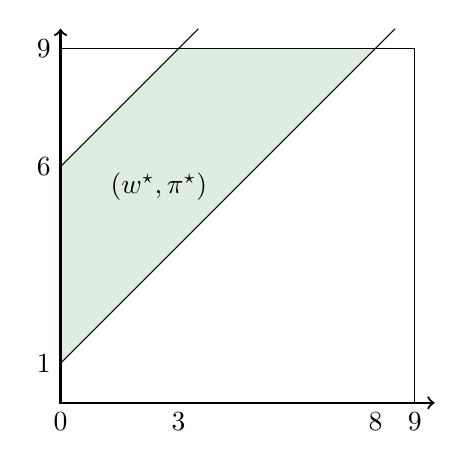
\begin{tikzpicture}[scale=0.5]
				\filldraw[ForestGreen!15] (0,1)--(0,6)--(3,9)--(8,9)--(0,1);
				\draw[thick,<->] (9.5,0)--(0,0)--(0,9.5);
				\draw (0,9)--(9,9)--(9,0);
				\node[left] at (0,1) {$1$};
				\node[left] at (0,6) {$6$};
				\node[left] at (0,9) {$9$};
				\node[below] at (0,0) {$0$};
				\node[below] at (3,0) {$3$};
				\node[below] at (8,0) {$8$};
				\node[below] at (9,0) {$9$};
				\draw (0,6)--(3.5,9.5);
				\draw (0,1)--(8.5,9.5);
				\node at (2.5,5.5) {$(w\opt,\pi\opt)$};
			\end{tikzpicture}
		\end{figure}
\end{example}


\begin{remark}
	No worker-firm pair can break off and do better on their own. What about larger coalitions of workers and firms?
\end{remark}

Define the total surplus any subset of workers can earn for themselves. Let $S \subseteq \mathcal{L} \cup \mathcal{F}$ be a set of workers and / or firms. If $S \subseteq \mathcal{L}$ or $S \subseteq \mathcal{F}$, let $v_P(S) = 0$. Otherwise, we define the total surplus that $S$ can earn for itself is
\begin{align*}
	v_P(S) = \max &\; \sum_{\ell,f \in S} v_{\ell f} \cdot x_{\ell f} \\ \st \qquad \sum_f x_{\ell f} &\le 1 \forall \ell \in S \\ \sum_\ell x_{\ell f} &\le 1 \forall f \in S \\ x_{\ell f} &\ge 0 \forall \ell,f \in S
\end{align*}
If $\sum_{\ell,f \in S} w_\ell + \pi_f < v_P(S)$, then $S$ can improve itself by breaking away. This matching problem defines a \blue{transferable utility game}.

\begin{definition}
	A payoff is in the \blue{core} of the matching game if no subset $S$ of individuals can improve by breaking away.
\end{definition}

\begin{theorem}
	Any stable payoff is a core payoff.
\end{theorem}
\begin{proof}
	Consider WLOG the coalition containing workers $1$ through $k$ and firms $1$ through $k$, and suppose that the optimal matching matches worker $i$ with firm $i$. For any stable payoff $(w\opt,\pi\opt)$  for the entire group, $w\opt_i + \pi\opt_i \ge v_{ii}$, so \[\sum_{i=1}^k w\opt_i + \pi_i\opt \ge \sum_{i=1}^k v_{ii} = v_P(S)\]so thus coalition $S$ cannot improve upon any stable payoff. The converse is obviously true.
\end{proof}

\begin{definition}
	A \blue{partially-ordered set (poset)} $(X,\succeq)$ is a set $X$ with a \blue{reflexive}, \blue{transitive}, and \blue{antisymmetric} binary relation $\succeq$. An element $x \in X$ is an \blue{upper bound} for $A \subseteq X$ if $x \succeq y$ for all $y \in A$, and $x$ is a \blue{supremum} for $A$ if it is an upper bound for $A$ and there is no other upper bound $x'$ with $x \succ x'$. Similarly for lower bounds.
	
	A \blue{lattice} is a poset in which each pair of elements $x,y \in X$ has a supremum $x \vee y \in X$ and an infimum $x \wedge y \in X$. A lattice is \blue{complete} if every subset $A \subseteq X$ has both a supremum and an infimum in $X$. 
	
	The sets $A \subseteq X$ is as large as the set $B \subseteq X$ in the \blue{strong set ordering}, denoted $A \sqsupseteq B$ if for all $x \in A$ and $y \in B$, $x \vee y \in A$ and $x \wedge y \in B$.
\end{definition}

Let $P$ denote the set of stable payoffs. Define $(w',\pi') \succeq (w'',\pi'')$ if for all $\ell$, $w_\ell' \ge w_\ell''$ and for all $f$, $\pi_f' \le \pi_f''$, each in the usual vector order. Then:

\begin{theorem}
	$(P,\succeq)$ is a complete lattice.
\end{theorem}
\begin{proof}
	Choose some $p' = (w',\pi')$ and $p'' = (w'',\pi'')$. First, we show that $p' \vee p''$ satisfies the dual constraints, meaning that 
	\begin{align*}
		w_\ell' &\ge v_{\ell f} - \pi'_f \\w_\ell'' &\ge v_{\ell f} - \pi''_f
	\end{align*}
	and so
	\[
	\max\{w_\ell',w_\ell''\} \ge \max\{ v_{\ell f} - \pi'_f, v_{\ell f} - \pi''_f\} = v_{\ell f} - \min\{\pi'_f,\pi''_f\}
	\]
	which means that $p\vee p' \ge v_{lf}$. A similar argument holds for $p \wedge p'$. Thus, the solutions are feasible, and complementary slackness holds the equations to equality as long as $\ell$ and $f$ are matched. Thus, $(P,\succeq)$ is a lattice. 
	
	Finally, we show that $P$ is complete. Let $A \subseteq P$ be a set of payoffs. We have that $\sup\{p : p \in A\}$ as $\bar{p}$ such that $\bar{w}_\ell = \sup\{w_\ell : p \in A\}$ and $\bar{\pi}_f = \inf\{\pi_f : p \in A\}$. It remains to show that $\bar{p} \in P$, \ie that $\bar{p}$ is an optimal solution to the dual problem. It suffices to show that $\bar{p}$ satisfies complementary slackness. Choose a matching $x$. For all $\varepsilon > 0$ there is a payoff in $A$ with $w^\varepsilon_\ell \le \bar{w}_\ell < w_\ell^\varepsilon + \varepsilon$, and $\pi_f^\varepsilon \ge \bar{\pi} > \pi_f^\varepsilon - \varepsilon$. Then \[v_{\ell f} - \varepsilon \le w_\ell^\varepsilon + \pi_f^\varepsilon - \varepsilon \le \bar{w}_\ell + \bar{\pi}_f\]Letting $\varepsilon \to 0$, we have that $\bar{w}_\ell + \bar{\pi}_f \ge v_{\ell f}$, so $\bar{p}$ is feasible. If $x_{\ell f} = 1$, then \[\bar{w}_\ell + \bar{\pi}_f \le w_\ell^\varepsilon + \pi_f^\varepsilon + \varepsilon \le v_{\ell f} - \varepsilon\]Again letting $\varepsilon \to 0$, we have that $\bar{w}_\ell + \bar{\pi}_f \le v_{\ell f}$. Thus, equality holds, which suffices to show that $\bar{p}$ satisfies complementary slackness.
\end{proof}

\begin{remark}
	There is a unique least wage payoff and a unique greatest wage payoff. The former is best for the firms and worst for the workers, the latter is best for the workers and worst for the firms. 
\end{remark}

Suppose we were given partial orders $\succ_\ell$ on workers and $\succ_f$ on firms. For instance, $\ell' \succ_\ell \ell''$ might mean that worker $\ell'$ is more skilled than worker $\ell''$, and $f' \succ_f f''$ might mean that any worker is more productive in firm $f'$ than in firm $f''$. 

\begin{proposition}
	Suppose that for all $\ell',\ell'',f',$ and $f''$, $\ell' \succ_\ell \ell''$ and $f' \succ_f f''$ means that $v_{\ell' f'} - v_{\ell'' f'} > v_{\ell' f''} - v_{\ell''f''}$. Then it cannot be the case that $\ell' \leftrightarrow f''$ and $\ell'' \leftrightarrow f'$. 
\end{proposition}
\begin{proof}
	If $v_{\ell' f'} - v_{\ell'' f'} > v_{\ell' f''} - v_{\ell''f''}$, then $v_{\ell' f'} + v_{\ell'' f''} > v_{\ell' f''} + v_{\ell'' f'}$, so we could increase surplus by changing the match.
\end{proof}
\begin{remark}
	The idea of matching bigger with bigger is called \blue{positive assortative matching}, and is due to \href{https://www.jstor.org/stable/1831130?seq=1}{Becker (1973)} on marriage. The property that the $v$ differences in $\ell$ are increasing in $f$ is called \blue{increasing differences}.
\end{remark}


\begin{question}
	How do wages and profits change with the surplus? Who gains and loses? 
\end{question}
\begin{remark}
	We use the framework of \blue{monotone comparative statics} to answer this question. Choose $\ell$ and $f$, and order $(w_\ell,\pi_f)$ as follows: \[(w,\pi) \succeq_{\ell f} (w',\pi') \Longleftrightarrow w_\ell + \pi_f \ge w'_\ell + \pi_f' \text{ and } w_\ell \ge w_\ell'\]Order remaining wages and profits with the usual $\ge$ order, and order $\reals^L_+ \times \reals^F_+$ with the product order:\[p \succeq p' \Longleftrightarrow (w_\ell ,\pi_f) \ge (w_{\ell'},\pi_{f'}) \text{ and } (w_\ell,\pi_f) \succeq_{\ell f} (w_{\ell'},\pi_{f'})\]
	
	Suppose $v_{\ell f}$ increases to $v_{\ell f}'$ holding all else fixed. There are three cases: (i) $x_{\ell f} = 1$, (ii) $x_{\ell f}' = 0$, and (iii) $x_{\ell f} = 0$ and $x_{\ell f} ' = 1$. However, there are really only two cases. The final case can be decomposed into regions where $\ell f$ is not an optimal match and regions where it is optimal. The two ranges intersect precisely at a point, where there are at least two optimal matches and all optimal matches have the same value. 
	
	\textbf{First Case.} If $\ell f$ is part of an optimal matching and $v_{\ell f}$ increases, it remains so. The set of dual solutions increases the payoffs to $\ell f$, and leaves all else unchanged. Take any dual solution to the new problem. Every other pair must be dividing up the value of their match, so the set of allocations of these surpluses in the old and new problem must be identical. And $\ell f$ must divide their surplus $v'_{\ell f}$, so their payoff set has increased in the strong set order. 
	
	\textbf{Second Case.} If $\ell f$ is out of the money, let $\sigma(\ell)$ denote $\ell$'s optimal match. Suppose $v_{\ell f}' > v_{\ell f}$, $\sigma(\ell) \ne f$, and $\sigma$ is optimal on the interval $[v_{\ell f} ,v'_{\ell f}]$, \emph{ceteris paribus}. Consider the minimal wage for $\ell$ and the maximal profit for $\sigma(\ell)$, so that $\underline{w}_\ell + \bar{\pi}_{\sigma(\ell)} = v_{\ell \sigma(\ell)}$.
	
	\begin{lemma}
		If $\underline{w}_\ell \ne 0$, there is a $f \in \sigma(\ell)$ such that\[\underline{w}_\ell + \bar{\pi}_f = v_{\ell f}\]and similarly for $\underline{\pi}_f$
	\end{lemma}
	\begin{proof}
		$(\underline{w}_\ell,\bar{\pi}_f)_{\ell f \in \mathcal{L} \cup \mathcal{F}}$ is a dual optimal payoff. Suppose FSOC the claim is false, so we have that for all $f \ne \sigma(\ell)$, $\underline{w}_\ell + \bar{\pi}_f \ge v_{\ell f} + \varepsilon$ for some $\varepsilon > 0$. Modifying the payoff by letting $w_\ell' = \underline{w}_\ell - \varepsilon'$ and $\bar{\pi}_{\sigma(\ell)}' = \bar{\pi}_{\sigma(\ell)} + \varepsilon'$ is feasible for any positive $\varepsilon' < \varepsilon$, and since the payoff has the same value this contradicts the minimality of $\underline{w}_\ell$. 
	\end{proof}
	
	We call this the \blue{opportunity constraint} for $\ell$. There is also an opportunity constraint for matching $f$ with $\sigma^{-1}(f)$.
	
	\begin{theorem}
		Suppose that $\ell g$ is the unique opportunity constraint for $\ell$. An increase in $w_{\ell g}$ raises $\underline{w}_\ell$ and decreases $\bar{\pi}_{\sigma(\ell)}$. A decrease in $v_{\ell g}$ lowers $\underline{w}_\ell$ and increases $\bar{\pi}_{\sigma(\ell)}$. 
	\end{theorem}
	\begin{proof}
		Replace $v_{\ell g}$ by $v'_{\ell g} > v_{\ell g}$ such that $\sigma$ still remains an optimal match. Then the binding opportunity constraint on $w_\ell$ is tighter, so $w_\ell$ increases. Replace $v_{\ell g}$ by $v'_{\ell g} < v_{\ell g}$ such that $\sigma$ still remains an optimal match. Then there is no binding opportunity constraint for $\ell$, and the argument in the above Lemma's proof shows that the new greatest lower bound $\underline{w}_\ell'$ on $w_\ell$ is less than $\underline{w}_\ell$, and that $\bar{\pi}'_{\sigma(\ell)} > \bar{\pi}_{\sigma(\ell)}$.
		
		Similarly, if $\ell g$ is the unique opportunity constraint for $f$, then raising $v_{\ell g}$ lowers $\underline{\pi}_f$ and raises $\bar{w}_{\sigma^{-1}(f)}$. Thus, if we increase $v_{\ell f}$ from a very low value for $f \ne \sigma(\ell)$, nothing happens until $\ell f$ becomes the opportunity constraint for $\ell$. Then $\underline{w}_\ell$ rises until it becomes optimal to assign $\ell$ to $f$. Then $\underline{w}_\ell$ holds constant. Along this same trajectory, $\bar{\pi}_{\sigma(\ell)}$ holds constant, then falls, then holds constant when it is no longer optimal to match $\ell$ with $\sigma(\ell)$. 
	\end{proof}
\end{remark}


\begin{model}
	\red{The Assignment Problem} The assignment problem is a one-sided version of the matching market. For example: the objective could be to match individuals to positions or houses or something similar. It can be set up as an LP the same way the matching market can. There are two versions:
	\begin{enumerate}
		\item \blue{Position constraints}, where the ``profits'' to positions are what the individuals pay for the position, and the ``wage'' is the remaining surplus, which they keep
		\item \blue{No constraints}, which we model as the case where there are more positions of each type than agents in the economy. Then the position price will be 0 and individuals keep all of the surplus. Here the focus is on self-selection and the match. An example of this is in \href{https://www.jstor.org/stable/2662082?seq=1}{Roy (1951)}.
	\end{enumerate}
\end{model}

\section{Matching Without Transfers}

There's a large literature in school choice, which is the broad problem we're trying to solve here. The history of schooling in America is one of neighborhood schools, but magnet schools started in New York City, and the problem was answered in Boston by using \href{https://www.jstor.org/stable/2312726?seq=1}{Gale \& Shapley (1962)}'s \blue{Deferred Acceptance Algorithm}.

\begin{model}
	\red{School Choice} We have a set $\mathcal{S}$ of students and a set $\mathcal{C}$ of schools. Each student $s \in \mathcal{S}$ has a strict preference order $\succ_s$ on $\mathcal{C}$, and each school $c \in \mathcal{C}$ has a strict preference order $\sqsupset_c$ on $\mathcal{S}$, and a capacity $q_c$. Finally, we have a \blue{matching} $\mu: \mathcal{S} \cup \mathcal{C} \to \mathcal{S} \cup \mathcal{C}$ such that (i) $|\mu(s)| = 1$ and $\mu(s) \in \mathcal{C}$; (ii) $\mu(c) \subset \mathcal{S}$; and (iii) $\mu(s) = c \Longleftrightarrow s \in \mu(c)$.
	
	\begin{definition}
		A matching $\mu$ is \blue{feasible} if no school is over capacity, so that $|\mu(c)| \le q_c$. Define the set of all \blue{preference profiles} that parents have $A^\mathcal{S}$, where for $N$ parents we have $(\succ_1,\succ_2,\dots,\succ_N)$. 
		
		Define a function $\phi: A^\mathcal{S} \to \mathcal{M}$, the set of all matchings, such that $\phi(\cdot)$ is, for all preference profiles $\phi$, feasible; such that for all $s$ $\mu(s) \succ_s \emptyset$ (\blue{individually rational}), and attains Pareto efficiency. Finally, we require that it attains the \blue{Elimination of Justified Envy}, which means that $\mu(t) \succ_s \mu(s) \Longrightarrow t \sqsupset_{\mu(t)} s$. This means that if $s$ prefers $t$'s match, then the school $t$ is matched to prefers $t$ to $s$. 
	\end{definition}
\end{model}

\begin{remark}
	Each mechanism introduces a game. Students may have an incentive to act strategically when submitting their preference order -- they might \emph{lie}! The game is that each student $s$ chooses a preference order $\succ_s' \in A$. Outcomes are $\phi\parl (\succ'_s)_{s \in \mathcal{S}}\parr \in \mathcal{M}$, and are ranked by each student according to $\unrhd_s$. 
\end{remark}

\begin{definition}
	A mechanism is \blue{strategy-proof} if each agent is always incentivized to tell the truth:\[\forall s \in \mathcal{S} , \forall \succ_{-s} \in \prod_{t \ne s}A_t , \forall \succ_s,\succ'_s \in A, \phi(\succ_{-s},\succ_s) \unrhd_s \phi(\succ_{-s},\succ'_s)\]
\end{definition}
\begin{algorithm}
	\red{Deferred Acceptance} Take the model as defined above, and implement the following:
	\begin{itemize}
		\item[\textbf{Step 1.}] Each student applies to her top school. Each school $c$ tentatively accepts all who apply up to $q_c$ (according to its ranking), rejecting the rest.
		\item[\textbf{Step $k$.}] Each student who was rejected at step $k-1$ applies to her top school among those to which she has not yet applied. Each school $c$ takes all of those tentatively accepted and the new applicants, ranks them according to $\sqsupset_c$, tentatively accepts the top $q_c$ students, and rejects the rest.
		\item[\textbf{Stop.}] The algorithm terminates when no student is rejected.
	\end{itemize}
\end{algorithm}
\begin{remark}
	We have the following results for deferred acceptance:
	\begin{enumerate}
		\item The algorithm will terminate. \\\begin{proof} Follows immediately from both sets being finite. \end{proof}
		\item The outcome is stable. \\\begin{proof} Suppose $s$ prefers $c$ to $\mu(s)$, and $c$ prefers $s$ to some matched $s'$. However, at some point $s$ would have applied to $c$, and $c$ would have had to held her over $s'$. This is a contradiction.\end{proof}
		\item The outcome is individually rational.\\\begin{proof} If a student reaches $\emptyset$, he applies, and since there is infinite capacity is accepted.\end{proof}
	\end{enumerate}
\end{remark}

\begin{theorem}
	The deferred acceptance algorithm matching is weakly preferred by every student to any other matching; that is, for every other stable matching, each student either gets the same or a less desirable match.
\end{theorem}
\begin{remark}
	This is called the \blue{student-optimal stable matching}.
\end{remark}
\begin{proof}
	(Intuitive) In the course of the deferred acceptance algorithm, no student is ever rejected by a school that would prefer her in any stable match.
\end{proof}

\begin{proof}
	(Actual) Say that school $c$ is \emph{possible} for student $s$ if they are matched in some stable matching. Assume that through the first $k-1$ steps nobody has been rejected by a possible school. Suppose that at step $k$, $s$ is rejected by $c$. Then $c$ has tentatively accepted a full quota of students $s_1,\dots,s_N$ from students with higher priorities. School $c$ is best for each $s_n$ among those schools that have not rejected her, and therefore each matching which gives $s \longleftrightarrow c$ will send some $s_n$ to a less desirable school. This matching is unstable because $(s_n,c)$ is a blocking pair. Thus at stage $k$, students are rejected by only schools impossible for them. The resulting assignment is therefore optimal.
\end{proof}

\begin{theorem}
	For stable matchings $\mu$ and $\nu$, the matching $\mu \vee \nu$ which assigns to each $s$ the better for her of $\mu(s)$ and $\nu(s)$ is a stable matching. So is $\mu \wedge \vee$ which assigns to each $s$ the worst of the two.
\end{theorem}
\begin{definition}
	A \blue{finite lattice} is a partially ordered set in which each pair has a least upper bound and a greatest lower bound. It is a \blue{distributive lattice} if $\wedge$ and $\vee$ distribute over each other. 
\end{definition}
\begin{remark}
	The implication here is that the set of stable matchings with these operations is a lattice, and it has a unique Pareto-best member.
\end{remark}

\begin{theorem}
	For any mechanism which gives the student-optimal stable matching for any problem, truth-telling is a dominant strategy for students.
\end{theorem}
\begin{proof}
	\href{https://www.jstor.org/stable/2321753?seq=1}{Dubins \& Freedman (1981)} and \href{https://wayback.archive-it.org/5456/20240920170030/http://www.eecs.harvard.edu/cs286r/courses/fall09/papers/roth.pdf}{Roth (1982)}.
\end{proof}

\section{Uncertainty}

\begin{definition}
	\blue{Commodities} are distributions on outcomes. \blue{Prices} are linear functionals of distributions -- integration of a function. Formally, commodities are random variables -- measurable functionals of states, while prices are linear functions on measurable functions -- measures on the state space.
\end{definition}
\begin{model}
	\red{The State Preference Model} Let $\mathcal{O}$ be the outcome space, $\mathcal{S}$ be the (finite) state space, $\mathcal{C}$ be the set of \blue{acts}, which are functions from states to outcomes, and $\succeq$ be a preference relation on acts. Some examples:
	\begin{align*}
		U(f) &= \min_s u(f(s)) &&\text{Maximin Utility} \\
		U(f) &= \sum_s u(f(s)) \mu(s) &&\text{Expected Utility} \\
		U(f) &= \min_{\mu \in \mathcal{P}}\sum_s u(f(s)) \mu(s) &&\text{Maximin Expected Utility} \\
		U(f) &= \frac{1}{1-\gamma} \int_\mathcal{P} \parl \sum_s u(f(s))\mu(s)\parr^{1-\gamma} \partial p(\mu) &&\text{The Smooth Model}
	\end{align*}
\end{model}

\begin{model}
	\red{The Two-Period Exchange Economy} $I$ traders live for two periods, $t = 0,1$. State $s \in S$ is revealed at the beginning of the second period. $L$ physical commodities are available at date 0 and states 1 through $S$. The consumption set for each trader is $\reals_+^{L(S+1)}$, and each trader has a strictly positive endowment vector $\omega^i \gg 0$ in the interior of the consumption set. Finally, each trader has beliefs $\pi^i$ and concave and increasing date $t$ payoff functions $u_t^i : \reals^L_+ \to \reals$, where \[U^i(x^i) = u^i(x^i_0) + \sum_{s=1}^S \pi_s^i u_1^i(x_s^i)\]
\end{model}

\begin{model}
	\red{The Arrow-Debreu Model} At date 0, traders trade current consumption bundles and contracts promising the delivery of $x_{s\ell}$ units of good $\ell$ if state $s$ occurs at time 1. \blue{Prices} are $\phi = (\phi_0,\dots,\phi_L) \in \reals^{L}_+ \setminus \{0\}$, and the \blue{Arrow-Debreu budget set} is\[B_{AD}(\phi,\omega^i) = \curll y \in \reals^{S(L+1)} : \sum_{s=0}^S \phi_s(y_s-\omega_s^i) = 0\curlr\]Equilibrium in the Arrow-Debreu model is a price $\phi$ and an allocation $x$ such that (i) each trader $i$ is maximizing $U^i(x^i)$ on $B_{AD}(\phi,\omega^i)$; and (ii) for all $s$ and $\ell$, $\sum_i x^i_{s\ell} - \omega^i_{s\ell} = 0$. 
	
	We can easily show that:
	\begin{enumerate}
		\item Equilibrium exists
		\item The First and Second Welfare Theorems apply
	\end{enumerate}
	However, what does Pareto optimality mean in this case?
	\begin{definition}
		Allocation $x$ is \blue{ex-ante Pareto preferred} to $y$ if for all $i$, $U^i(x^i) \ge U^i(y^i)$, with strict inequality for some $i$.
		
		Allocation $x$ is \blue{ex-post Pareto preferred} to $y$ if for all $i$ and for all $s \ge 0$, $u^i(x^i_s) \ge u^i(y^i_s)$ with strict inequality for some $i$.
	\end{definition}
	
	\begin{theorem}
		If for all $i$ and all $s \ge 1$, $\pi_i(s) \ge 0$, then if $x$ is ex-ante Pareto preferred to $y$, then $x$ is ex-post Pareto preferred to $y$.
	\end{theorem}
	\begin{remark}
		The converse does not hold here.
	\end{remark}
\end{model}

\begin{model}
	\red{The Radner Model} Traders can trade $L$ physical commodities at both time 0 and in each time 1 state $s \in S$ spot market, and $J$ assets. Asset $j$ is a promise to pay to its holder $a_s^j$ units of good 1 in state $s$. The asset return matrix is the $|S| \times J$ matrix $A$ with rows $A_s$. The vector of state-contingent returns from portfolio $z \in \reals^J$ is $Az$. Note that the set of feasible portfolios is unbounded -- $z_j < 0$ is a \blue{short / sale position}, while $z_j > 0$ is a \blue{long / purchase position}. Prices in the Radner model are spot prices $p \in \reals^{L(S+1)}_+$ and asset prices $q \in \reals^J$. 
	
	We can illustrate this with the \blue{Date-Event Tree}:
	\begin{figure}[H]
		\centering
		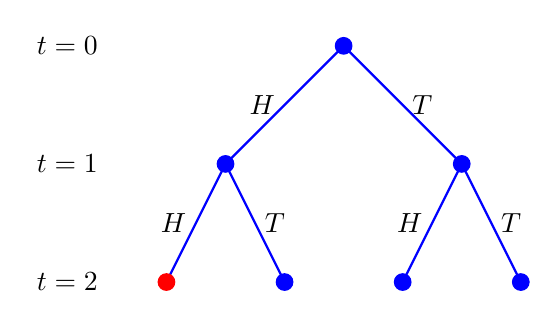
\begin{tikzpicture}[scale=1.5]
			\draw[blue,thick](-1.5,-2)--(-1,-1)--(-0.5,-2);
			\draw[blue,thick](1.5,-2)--(1,-1)--(0.5,-2);
			\draw[blue,thick] (-1,-1)--(0,0)--(1,-1);
			
			\filldraw[blue] (0,0) circle(2pt);
			\filldraw[blue] (1,-1) circle(2pt);
			\filldraw[blue] (-1,-1) circle(2pt);
			\filldraw[red] (-1.5,-2) circle(2pt);
			\filldraw[blue] (-.5,-2) circle(2pt);
			\filldraw[blue] (.5,-2) circle(2pt);
			\filldraw[blue] (1.5,-2) circle(2pt);
			\node[left] at (-0.5,-0.5){$H$};
			\node[right] at (0.5,-0.5) {$T$};
			\node[left] at (-1.25,-1.5){$H$};
			\node[right] at (-0.75,-1.5) {$T$};
			\node[left] at (0.75,-1.5){$H$};
			\node[right] at (1.25,-1.5) {$T$};
			
			\node[left] at (-2,0) {$t=0$};
			\node[left] at (-2,-1) {$t=1$};
			\node[left] at (-2,-2) {$t=2$};
		\end{tikzpicture}
	\end{figure}
	Each node is a spot market, and each edge is a state. The \textcolor{red}{red} node is at the spot market after two $H$ states have been realized. People trade goods \textbf{at} spot markets, and they trade assets \textbf{between} spot markets.
	
	The \blue{Radner budget set} is \[B_R(p,q,\omega^i) = \Bigg\{ (y,z) \in \reals_+^{L(S+1)} \times \reals^J : p_0 \cdot y_0 + q\cdot z = p_0 \cdot \omega_0^i; \; p_s \cdot y_s = p_s\cdot\omega_s^i + p_{s1}\cdot A_s\cdot z \forall s \in S\Bigg\}\]
	Note that this budget set is homogeneous of degree zero in all $p_s$, so we can take the spot market prices for numeraire to all be 1 WLOG. Formally, for $s \in S, p_{1s}=1$.
	
	\begin{definition}
		\blue{Equilibrium} in the Radner model is a vector of spot prices $p$, asset prices $q$, a commodity allocation $x$, and an asset allocation $z$ such that:
		\begin{enumerate}
			\item Each trader $i$ is maximizing $U^i(x^i)$ on $B_R(p,q,\omega^i)$
			\item For all $s$ and $\ell$, $\sum_i x_{s\ell}^i - \omega_{s\ell}^i = 0$
			\item $\sum_j z^j =0$
		\end{enumerate}
	\end{definition}
	
	\begin{remark}
		If there is a portfolio with a semi-positive return vector, then some spot-market budget sets are unbounded. Equilibrium requires that no such portfolio exists, which may restrict asset prices. Let \[M = \matrixc{-q \\ A}\]with column space $\langle M \rangle$. The \blue{no-arbitrage condition} is satisfied if there is no portfolio $z$ such that $Mz > 0$. That is, \[\langle M \rangle \cap \reals^{S+1}_+ = \{0\}\]
	\end{remark}
\end{model}

\begin{theorem}
	The no arbitrage condition is satisfied if and only if there is a $\tilde{\pi} \gg 0$ such that $\tilde{\pi}\cdot M = 0$
\end{theorem}
\begin{proof}
	The no-arbitrage theorem is a theorem of the alternative. Let $\Delta$ denote the set of $y \in \reals^{S+1}_+$ such that $\sum_n y_n = 1$. If $Mz > 0$ has a solution, it will have one in $\Delta$. First, a preliminary result:
	\begin{lemma}\red{Separating Hyperplane Theorem}
		If $A,B \subseteq \reals^m$ are convex, $A$ closed, $B$ compact, then there is a $\pi$ that separates them, meaning that \[\sup_{a\in A} \pi \cdot a < \inf_{b\in B} \pi \cdot b\]
	\end{lemma}
	\begin{proof} In math notes, in full. Too long to reprint here.
	 \end{proof}
	 
	 ($\Leftarrow$) If $\tilde{\pi}M = 0$, then $\tilde{\pi}Mz = 0 \forall z$. Since $\tilde{\pi} \gg 0$, $Mz \not> 0$. 
	 
	 ($\Rightarrow$) Suppose that $\langle M \rangle \cap \reals^{S+1}_+ = \{0\}$. Suppose that $D = \{y : y = Mz, z \in \reals^J\}$. The no-arbitrage condition says that $\Delta \cap D = \emptyset$, and the lemma says that there is a $\pi$ that separates them. 
	 
	 Suppose that $\pi \le 0$. Then the infimum over $\Delta$ is weakly negative, but $0 \in D$, which is a contradiction. Thus, $\pi \gg 0$. Next suppose that $\pi d \ne 0$ for some $d \in D$. Then there is a $z \in \reals^J$ such that $\pi M z \ne 0$, so expanding positively or negatively as needed we have that $\sup_{d\in D} \pi d = +\infty$, which is another contradiction.
\end{proof}



\begin{remark}
	If there is such a $\tilde{\pi}$, WLOG let the first component be 1. Let\[P(q) = \curll \pi \in \reals^S_{++} : (1,\pi)\cdot M = 0\curlr\]Then $\pi \in P(q)$ if and only if\[q^j = \pi_1a_q^j + \cdots + \pi_Sa^j_S\]Any member of $P(q)$ is called a \blue{state price vector}. From Rank-Nullity, $\dim P(q) = S - \rank A$, so $\pi$ will be unique if and only if $\rank A = S$. In this case, markets are said to be \blue{complete}. 
\end{remark}

\begin{definition}
	An asset is \blue{redundant} if $A^j = \sum_{k\ne j} \alpha_k A^k$. To see why, note that each $q_k = \pi A^k$, so\[q_j = \pi \sum_{k\ne j} \alpha_k A^k = \sum_{k\ne j} \alpha_k \pi A^k = \sum_{k \ne j} \alpha_k q_k\]An \blue{Arrow security} is an asset that pays off 1 in a single state $s$ and 0 otherwise. If $\pi$ is a state price vector, then $q = \pi$ is the price vector of Arrow securities.
\end{definition}


\begin{theorem}\red{Arrow's Other Theorem} 
	Suppose that $\rank A = S$. Then:
	\begin{enumerate}
		\item Suppose Radner prices are $(p,q)$ with state prices $\pi$, and define $\phi_0 = p_0$, and for $s \ge 1$, $\phi_{s\ell} = \pi_s \frac{p_{s\ell}}{p_{s1}}$. Then $(x,z) \in B_R(p,q,\omega^i)$ if and only if $x \in B_{AD}(p,\omega^i)$
		\item Suppose Arrow-Debreu prices are $\phi$, and define $p_0 = \phi_0$, $\pi_s = \phi_{s1}$, $p_{s\ell} = \frac{\phi_{s\ell}}{\phi_{s1}}$, and $q = \pi A$. Then $x \in B_{AD}(\phi,\omega^i)$ if and only if there exists $z$ such that $(x,z) \in B_R(p,q,\omega^i)$. 
	\end{enumerate}
\end{theorem}
\begin{proof}
	The proof is just algebra. It's fully in \href{https://www.jstor.org/stable/2296188?seq=1}{Arrow (1952)} (\emph{n.b.} translated 1964).
\end{proof}

\begin{remark}
	The implications here are that:
	\begin{enumerate}
		\item When markets are complete, Radner and Arrow-Debreu equilibrium commodity allocations are identical
		\item Prices of either equilibrium type can be derived from the other
		\item All Radner equilibria are Pareto optimal
	\end{enumerate}
\end{remark}

\begin{question}
	What happens when markets are incomplete?
\end{question}

We have first order conditions in the Radner market that give us (i) multipliers $\lambda_s^i$ for constraint $s$, where $s = 0,1,\dots,S$; (ii) slackness conditions for all $s$ and $\ell$, $D_{s\ell} U^i(x^i) - \lambda_s^i p_{s\ell} = 0$; and (iii) slackness conditions for all $j$ where $-\lambda_0^i q_j+\sum_s \lambda_s^i a_s^j = 0$. Additionally, the Radner budget constraint must be satisfied, and we must have that $x^i,\lambda^i \gg 0$.

When markets are complete, equilibrium is optimal. This is not the case when markets are incomplete. 

\begin{remark}
	We can easily derive optimality of equilibrium with complete markets from the first order conditions, which tell us that within a state \[\frac{D_{s\ell} U^i(x^i)}{D_{sm}U^i(x^i)} = \frac{p_{s\ell}}{p_{sm}}\]meaning that the marginal rates of substitution between goods in the same state are equal across individuals. Across states, we have that \[\frac{D_{s\ell} U^i(x^i)}{D_{tm}U^i(x^i)} = \frac{\lambda_s^i}{\lambda_t^i} \frac{p_{s\ell}}{p_{tm}} \qquad \text{ and } \qquad \frac{\lambda_s^i}{\lambda_t^i} = \frac{q_s}{q_t}\]meaning that marginal rates of substitution between goods in different states equal a constant times the marginal rate of substitution between the numeraires in different states. With complete markets, they are also equal. Since individuals marginal rates of substitution of wealth across states are pinned down by the asset price ratios, all marginal rates of substitution are equal and equilibrium is Pareto optimal. 
\end{remark}

\begin{remark}
As an example of what happens when markets are incomplete, consider a market where the only asset is a bond but there are at least two states. The bond pays off one unit of numeraire in every state. Our first order conditions are, for each state $s$,\[D_{s\ell}U^i(x^i) - \lambda_s^i p_{s\ell} = 0 \qquad \text{ and } \qquad -\lambda_0^i q^1 + \sum_{s=1}^S \lambda_s^i = 0\]Thus, any vector \[\pi^i = \parl \frac{\lambda_1^i}{\lambda_0^i},\cdots,\frac{\lambda_s^i}{\lambda_0^i}\parr\]is a \blue{state price vector}. However, since $\rank A < S$, state prices are not unique, so there is no force equilibrating marginal rates of substitution across different states.
\end{remark}

\begin{remark}
	Market incompleteness causes issues for the existence of equilibrium. \href{https://www.jstor.org/stable/1909407}{Radner (1973)} showed equilibrium existence with an additional assumption that bounded the set of allowable asset positions; \href{https://www.sciencedirect.com/science/article/pii/0022053175900289}{Hart (1975)} discussed non-existence and other issues with the Arrow-Debreu world that arise in such models; and \href{https://www.jstor.org/stable/41953246?seq=1}{Polemarchakis (1990)} has a good summary discussion of existence, especially regarding how existence is achieved in some asset structures.
\end{remark}
































\end{document}